\documentclass[12pt,a4paper]{article}

\usepackage[utf8]{inputenc}
\usepackage[T5]{fontenc}
\usepackage[vietnamese]{babel}
\usepackage{geometry}
\usepackage{amsmath,amssymb}
\usepackage{graphicx}
\usepackage{array}
\usepackage{booktabs}
\usepackage[hypertexnames=false]{hyperref}
\usepackage{fancyhdr}
\usepackage{titlesec}
\usepackage{setspace}
\usepackage[numbers]{natbib}
\usepackage{listings}
\usepackage{xcolor}

\geometry{margin=2.5cm}
\setlength{\parindent}{0pt}
\setstretch{1.0} % Giãn cách giữa các dòng trong cùng đoạn
\setlength{\parskip}{0.35\baselineskip} % Giãn cách giữa các đoạn
\setlength{\headheight}{15pt}

\lstdefinestyle{pseudocode}{
    basicstyle=\ttfamily\small,
    breaklines=true,
    frame=single,
    numbers=left,
    numberstyle=\tiny,
    keywordstyle=\bfseries,
    commentstyle=\itshape,
    showstringspaces=false,
    tabsize=4
}

\pagestyle{fancy}
\fancyhf{}
\lhead{Nhập môn Phân tích độ phức tạp thuật toán}
\rhead{XGBoost}
\renewcommand{\headrulewidth}{0.4pt}
\renewcommand{\footrulewidth}{0.4pt}

\titleformat{\section}{\Large\bfseries}{\thesection}{1em}{}
\titleformat{\subsection}{\large\bfseries}{\thesubsection}{1em}{}

\begin{document}

\begin{titlepage}
  \centering
  % \vspace*{1cm}

  {\Large\textbf{TRƯỜNG ĐẠI HỌC KHOA HỌC TỰ NHIÊN, ĐHQG-HCM}\\}
  \vspace{0.4cm}
  {\large\textbf{KHOA CÔNG NGHỆ THÔNG TIN}\\}

  \vspace{1.6cm}

  {\Large\textbf{BÁO CÁO MÔN HỌC}\\}
  \vspace{0.5cm}
  {\Large\textbf{NHẬP MÔN PHÂN TÍCH ĐỘ PHỨC TẠP THUẬT TOÁN}\\}

  \vspace{1.0cm}

  {\Huge\textbf{CHỦ ĐỀ: XGBOOST}\\}

  \vfill

  \begin{tabular}{>{\bfseries}l l}
    Môn học: & Nhập môn Phân tích độ phức tạp thuật toán \\
    Chủ đề: & XGBoost \\
  \end{tabular}

  \vspace{0.8cm}

  \begin{tabular}{>{\bfseries}l l}
    \multicolumn{2}{l}{\textbf{Thành viên thực hiện:}} \\
    Trần Minh Hiếu Học & 23120006 \\
    Phan Trọng Đài & 23120026 \\
    Trần Đăng Khoa & \textit{chưa cung cấp} \\
    Lê Văn Trường & 23120181 \\
    Đinh Nho Hoàng & 23120420\\
  \end{tabular}

  \vspace{0.8cm}

  \begin{tabular}{>{\bfseries}l l}
    \multicolumn{2}{l}{\textbf{Giảng viên hướng dẫn:}} \\
    Thầy Cấn Trần Thành Trung & \\
    Thầy Lê Phúc Lữ & \\
  \end{tabular}

  \vfill

  {\large TP. Hồ Chí Minh, \today}
\end{titlepage}

\pagenumbering{roman}
\tableofcontents
\newpage

\pagenumbering{arabic}

\section{Introduction}

\subsection{Bối cảnh}

Trong các bài toán học máy hiện đại, dữ liệu thường có kích thước lớn, số lượng đặc trưng cao và quan hệ giữa các biến đầu vào có thể rất phức tạp. Các mô hình tuyến tính có ưu điểm là đơn giản, dễ huấn luyện và dễ diễn giải, nhưng thường gặp hạn chế khi dữ liệu có quan hệ phi tuyến hoặc có nhiều tương tác giữa các đặc trưng. Trong bối cảnh đó, các mô hình dựa trên cây quyết định trở thành một hướng tiếp cận quan trọng nhờ khả năng mô hình hóa quan hệ phi tuyến, xử lý linh hoạt cả dữ liệu số lẫn dữ liệu phân loại, đồng thời vẫn giữ được mức độ diễn giải tương đối trực quan \cite{breiman1984classification}.

Tuy nhiên, một cây quyết định đơn lẻ thường có khả năng dự đoán chưa đủ mạnh và dễ bị overfitting nếu cây phát triển quá sâu. Vì vậy, các phương pháp học tổ hợp được sử dụng để kết hợp nhiều mô hình yếu thành một mô hình mạnh hơn. Trong nhóm phương pháp này, Bagging tập trung giảm phương sai bằng cách huấn luyện nhiều mô hình độc lập \cite{breiman1996bagging}, trong khi Boosting xây dựng các mô hình theo cách tuần tự, trong đó mô hình sau tập trung cải thiện lỗi của mô hình trước. Gradient Boosting là một trong những phương pháp Boosting quan trọng, đặt quá trình học trong góc nhìn tối ưu hàm mất mát theo hướng gradient \cite{friedman2001gradient}.

XGBoost, viết tắt của Extreme Gradient Boosting, là một hệ thống gradient tree boosting được thiết kế với mục tiêu vừa đạt hiệu quả dự đoán cao, vừa có khả năng mở rộng trên dữ liệu lớn. Theo Chen và Guestrin, XGBoost không chỉ là một mô hình học máy, mà còn là một hệ thống tối ưu toàn diện cho quá trình huấn luyện cây tăng cường. Các cải tiến quan trọng của XGBoost bao gồm regularization, approximate split finding, weighted quantile sketch, sparsity-aware split finding, column block structure, cache-aware access và out-of-core computation \cite{chen2016xgboost}.

Dưới góc nhìn của môn Nhập môn Phân tích độ phức tạp thuật toán, điểm đáng quan tâm của XGBoost không chỉ nằm ở độ chính xác dự đoán, mà còn nằm ở cách hệ thống này giảm chi phí tính toán trong quá trình xây dựng cây. Trong đó, bài toán tìm điểm phân tách tốt nhất, hay còn gọi là \textit{split finding}, là một trong những bước tốn thời gian nhất. Do đó, việc phân tích XGBoost cũng là cơ hội để thấy rõ cách các ý tưởng thuật toán và cấu trúc dữ liệu có thể cải thiện hiệu năng của một hệ thống học máy thực tế.

\subsection{Mục tiêu báo cáo}

Báo cáo này tập trung tìm hiểu XGBoost dưới góc nhìn thuật toán và độ phức tạp. Các mục tiêu chính gồm:

\begin{itemize}
    \item Trình bày nền tảng về cây quyết định, học tổ hợp, Boosting và Gradient Boosting.
    \item Giải thích cách XGBoost mở rộng Gradient Boosting thông qua regularization và khai triển Taylor bậc hai.
    \item Phân tích công thức toán học cốt lõi của XGBoost, bao gồm gradient, Hessian, trọng số lá và split gain.
    \item Tìm hiểu các thuật toán tìm split trong XGBoost, bắt đầu từ Exact Greedy Split.
    \item Phân tích độ phức tạp của các bước xây dựng cây, đặc biệt là chi phí tìm split.
\end{itemize}

Trọng tâm của báo cáo là làm rõ vì sao việc tìm split là nút thắt tính toán trong các mô hình cây, và XGBoost đã sử dụng những kỹ thuật thuật toán nào để giảm chi phí này.

\subsection{Vai trò của Split Finding trong độ phức tạp thuật toán}

Trong quá trình xây dựng cây quyết định, tại mỗi node, thuật toán cần chọn một đặc trưng và một ngưỡng phân tách sao cho chất lượng mô hình được cải thiện nhiều nhất. Nếu dữ liệu có $n$ mẫu và $d$ đặc trưng, việc duyệt qua nhiều ngưỡng phân tách trên từng đặc trưng có thể dẫn đến chi phí rất lớn.

Đối với một cây đơn lẻ, chi phí tìm split đã là một thành phần quan trọng. Với XGBoost, quá trình này còn được lặp lại qua nhiều cây trong nhiều vòng boosting. Nếu số cây là $K$ và độ sâu tối đa của mỗi cây là $h$, thì chi phí tìm split có thể trở thành thành phần chi phối thời gian huấn luyện.

Do đó, phân tích XGBoost dưới góc nhìn độ phức tạp thực chất là phân tích cách hệ thống này tối ưu quá trình tìm split. Các kỹ thuật như Column Block Structure, Approximate Split Finding, Weighted Quantile Sketch và Sparsity-aware Split Finding đều hướng đến mục tiêu chung: giảm số lần sắp xếp, giảm số candidate split cần xét, tận dụng dữ liệu thưa và cải thiện khả năng mở rộng của quá trình huấn luyện \cite{chen2016xgboost}.
\section{Decision Tree}

\subsection{Khái niệm}

Cây quyết định là một mô hình học máy có cấu trúc dạng cây, trong đó quá trình dự đoán được thực hiện thông qua một chuỗi các phép kiểm tra trên đặc trưng đầu vào. Mỗi nút trong biểu diễn một điều kiện phân tách, mỗi cạnh tương ứng với kết quả của điều kiện đó, và mỗi nút lá chứa dự đoán cuối cùng của mô hình \cite{breiman1984classification}.

Với bài toán phân loại, nút lá thường chứa nhãn lớp hoặc phân phối xác suất trên các lớp. Với bài toán hồi quy, nút lá thường chứa một giá trị số, chẳng hạn trung bình của các giá trị mục tiêu trong node đó. Nhờ cấu trúc phân nhánh rõ ràng, cây quyết định có ưu điểm là dễ diễn giải và có thể mô hình hóa các quan hệ phi tuyến giữa đặc trưng và nhãn.

Một cây quyết định gồm các thành phần chính:

\begin{itemize}
    \item \textbf{Root node}: nút gốc, chứa toàn bộ tập dữ liệu ban đầu.
    \item \textbf{Internal node}: nút trong, chứa một điều kiện phân tách.
    \item \textbf{Split}: phép chia một tập mẫu thành các tập con dựa trên một đặc trưng và một ngưỡng.
    \item \textbf{Threshold}: ngưỡng dùng để quyết định mẫu đi sang nhánh trái hay nhánh phải.
    \item \textbf{Leaf node}: nút lá, nơi mô hình đưa ra dự đoán.
\end{itemize}

Ví dụ, một node có thể có điều kiện:

\[
x_j \leq s,
\]

trong đó $x_j$ là giá trị của đặc trưng thứ $j$, còn $s$ là threshold. Khi đó, một mẫu dữ liệu sẽ được đưa sang nhánh trái nếu $x_j \leq s$, và sang nhánh phải nếu $x_j > s$. Quy ước này cũng là quy ước được dùng trong phần code minh họa của báo cáo.

\subsection{Minh họa cấu trúc cây}

Một cây quyết định nhị phân đơn giản có thể được minh họa như sau:

\begin{figure}[h]
    \centering
    \fbox{
    \begin{minipage}{0.75\linewidth}
    \centering
    \vspace{0.2cm}
    Root: $x_1 < 5$?\\[0.2cm]
    $\swarrow$ \hspace{3cm} $\searrow$\\
    Leaf: class A \hspace{1.5cm} Internal: $x_2 < 3$?\\
    \hspace{4.2cm} $\swarrow$ \hspace{1.5cm} $\searrow$\\
    \hspace{3.2cm} Leaf: class B \hspace{0.5cm} Leaf: class C
    \vspace{0.2cm}
    \end{minipage}
    }
    \caption{Minh họa một cây quyết định nhị phân đơn giản.}
    \label{fig:decision_tree_example}
\end{figure}

Trong ví dụ trên, mỗi sample bắt đầu từ root node, đi qua một số điều kiện phân tách, sau đó kết thúc tại một leaf node. Dự đoán của mô hình chính là giá trị được lưu tại leaf node đó.

\subsection{Tiêu chí phân tách}

Mục tiêu của quá trình xây dựng cây là chọn các split sao cho các mẫu trong cùng một nút lá càng đồng nhất càng tốt. Với bài toán phân loại, một node được xem là tốt nếu phần lớn mẫu trong node thuộc cùng một lớp. Với bài toán hồi quy, một node được xem là tốt nếu các giá trị mục tiêu trong node ít biến thiên.

Một số tiêu chí phân tách phổ biến gồm:

\begin{itemize}
    \item \textbf{Gini impurity}: thường dùng trong bài toán phân loại.
    \item \textbf{Entropy và Information Gain}: đo mức độ giảm bất định sau khi phân tách.
    \item \textbf{Mean Squared Error}: thường dùng trong bài toán hồi quy.
\end{itemize}

Với bài toán phân loại, Gini impurity của một node được định nghĩa là:

\[
Gini = 1 - \sum_{c=1}^{C} p_c^2,
\]

trong đó $p_c$ là tỷ lệ mẫu thuộc lớp $c$ trong node, và $C$ là số lớp.

Với bài toán hồi quy, một tiêu chí phổ biến là tổng sai số bình phương trong các node con:

\[
MSE = \frac{1}{n}\sum_{i=1}^{n}(y_i - \bar{y})^2,
\]

trong đó $\bar{y}$ là giá trị trung bình của các nhãn trong node.

Trong XGBoost, tiêu chí chọn split không trực tiếp dùng Gini hay MSE như cây quyết định truyền thống. Thay vào đó, XGBoost sử dụng một công thức gain được suy ra từ hàm mục tiêu có regularization và khai triển Taylor bậc hai \cite{chen2016xgboost}. Điều này giúp tiêu chí phân tách của XGBoost gắn trực tiếp với mục tiêu tối ưu của mô hình.

\subsection{Mã giả xây dựng cây quyết định}

Quá trình xây dựng cây quyết định thường được thực hiện theo cách đệ quy. Tại mỗi node, thuật toán tìm split tốt nhất, chia dữ liệu thành hai tập con, sau đó tiếp tục xây dựng cây trên từng tập con.

\begin{lstlisting}[style=pseudocode, caption={Mã giả xây dựng cây quyết định}, label={lst:decision_tree}]
BuildTree(D, depth):
    if stopping_condition(D, depth):
        return Leaf(prediction)

    best_split = None
    best_score = -infinity

    for each feature j:
        for each threshold s:
            split D into D_left and D_right
            score = evaluate_split(D_left, D_right)

            if score > best_score:
                best_score = score
                best_split = (j, s)

    split D using best_split into D_left and D_right
    create internal node using best_split
    left_child = BuildTree(D_left, depth + 1)
    right_child = BuildTree(D_right, depth + 1)

    return node
\end{lstlisting}

Điểm quan trọng trong thuật toán trên là vòng lặp tìm \texttt{best\_split}. Đây chính là phần tốn kém nhất, vì thuật toán phải xét nhiều đặc trưng và nhiều threshold khác nhau.

\subsection{Độ phức tạp}

Giả sử tại một node có $n$ mẫu và $d$ đặc trưng. Để tìm split tốt nhất, thuật toán cần xét các threshold trên từng đặc trưng.

Nếu mỗi đặc trưng là liên tục, một cách làm phổ biến là sắp xếp các mẫu theo giá trị của đặc trưng đó. Chi phí sắp xếp một đặc trưng là:

\[
O(n \log n).
\]

Với $d$ đặc trưng, chi phí sắp xếp là:

\[
O(dn \log n).
\]

Sau khi sắp xếp, thuật toán có thể quét tuyến tính để đánh giá các split candidate, với chi phí:

\[
O(dn).
\]

Vì vậy, chi phí tại một node có thể được ước lượng là:

\[
O(dn \log n + dn) = O(dn \log n).
\]

Nếu cây có độ sâu tối đa là $h$, việc tìm split sẽ được lặp lại ở nhiều node. Trong thực tế, tổng chi phí phụ thuộc vào cách dữ liệu được chia qua các node. Tuy nhiên, có thể thấy rằng thao tác tìm split là thành phần chi phối chi phí xây dựng cây.

Đây cũng là lý do các phần sau của báo cáo tập trung vào các kỹ thuật tối ưu split finding trong XGBoost.

\section{Ensemble Learning}

\subsection{Ý tưởng tổng quát}

Ensemble Learning, hay học tổ hợp, là nhóm phương pháp kết hợp nhiều mô hình cơ sở để tạo ra một mô hình tổng hợp mạnh hơn. Thay vì chỉ dựa vào một mô hình đơn lẻ, ensemble huấn luyện nhiều mô hình yếu hoặc mô hình cơ sở, sau đó kết hợp dự đoán của chúng để đưa ra kết quả cuối cùng.

Một mô hình yếu là mô hình có khả năng dự đoán tốt hơn ngẫu nhiên nhưng chưa đủ mạnh nếu sử dụng riêng lẻ. Trực giác của ensemble là nếu các mô hình thành phần mắc lỗi theo những cách khác nhau, việc kết hợp chúng có thể giúp giảm lỗi tổng thể và cải thiện khả năng khái quát hóa.

Với bài toán phân loại, kết quả cuối cùng thường được lấy bằng voting:

\[
\hat{y} = \mathrm{majority\_vote}(f_1(x), f_2(x), \ldots, f_K(x)).
\]

Với bài toán hồi quy, kết quả cuối cùng có thể là trung bình hoặc tổng có trọng số của các mô hình thành phần:

\[
\hat{y} = \frac{1}{K}\sum_{k=1}^{K} f_k(x).
\]

Riêng trong các mô hình Boosting, các mô hình thành phần thường được cộng dồn tuần tự:

\[
\hat{y} = \sum_{k=1}^{K} f_k(x).
\]

Cách biểu diễn này là nền tảng cho Gradient Boosting và XGBoost, trong đó mỗi cây mới được thêm vào nhằm cải thiện mô hình hiện tại.

\subsection{Bagging}

Bagging, viết tắt của Bootstrap Aggregating, là một kỹ thuật ensemble trong đó nhiều mô hình được huấn luyện độc lập trên các tập dữ liệu con được lấy mẫu lại từ tập dữ liệu ban đầu \cite{breiman1996bagging}.

Quy trình tổng quát của Bagging gồm:

\begin{enumerate}
    \item Tạo nhiều tập dữ liệu con bằng cách lấy mẫu có hoàn lại từ tập train.
    \item Huấn luyện một mô hình riêng trên mỗi tập dữ liệu con.
    \item Kết hợp dự đoán của các mô hình bằng voting hoặc averaging.
\end{enumerate}

Random Forest là một ví dụ tiêu biểu của Bagging với cây quyết định. Mỗi cây được huấn luyện trên một tập mẫu khác nhau và thường chỉ xét một tập con các đặc trưng tại mỗi split. Cơ chế này giúp các cây trong ensemble đa dạng hơn.

Ưu điểm chính của Bagging là giảm variance. Nếu một cây quyết định đơn lẻ dễ bị overfitting do quá nhạy với dữ liệu huấn luyện, thì việc trung bình hóa nhiều cây có thể giúp mô hình ổn định hơn.

\subsection{Boosting}

Boosting là một kỹ thuật ensemble trong đó các mô hình được huấn luyện tuần tự. Khác với Bagging, các mô hình trong Boosting không độc lập với nhau. Mô hình sau được xây dựng dựa trên lỗi hoặc tín hiệu tối ưu còn lại của mô hình trước.

Ý tưởng tổng quát có thể viết dưới dạng mô hình cộng dồn:

\[
F_K(x) = f_1(x) + f_2(x) + \cdots + f_K(x),
\]

trong đó $f_k$ là mô hình yếu thứ $k$.

Trong Boosting, mỗi mô hình mới không cố gắng giải quyết toàn bộ bài toán từ đầu. Thay vào đó, nó tập trung cải thiện phần mà mô hình hiện tại chưa dự đoán tốt. Vì vậy, Boosting thường có khả năng giảm bias tốt và tạo ra mô hình dự đoán mạnh từ nhiều mô hình yếu.

Gradient Boosting là một dạng Boosting quan trọng, trong đó mô hình mới được học theo hướng làm giảm hàm mất mát bằng gradient \cite{friedman2001gradient}. XGBoost tiếp tục mở rộng hướng tiếp cận này bằng cách bổ sung regularization, đạo hàm bậc hai và nhiều tối ưu thuật toán \cite{chen2016xgboost}.

Một số mô hình Boosting phổ biến gồm AdaBoost, Gradient Boosting, XGBoost, LightGBM và CatBoost.

\subsection{So sánh Bagging và Boosting}

\begin{table}[htbp]
    \centering
    \caption{So sánh Bagging và Boosting}
    \label{tab:bagging_boosting}
    \begin{tabular}{p{3.2cm}p{6.0cm}p{6.0cm}}
        \toprule
        \textbf{Tiêu chí} & \textbf{Bagging} & \textbf{Boosting} \\
        \midrule
        Cách huấn luyện 
        & Các mô hình được huấn luyện song song và tương đối độc lập 
        & Các mô hình được huấn luyện tuần tự, mô hình sau phụ thuộc vào mô hình trước \\

        Mục tiêu chính 
        & Giảm variance và tăng độ ổn định 
        & Giảm bias và tối ưu lỗi dự đoán \\

        Ví dụ tiêu biểu 
        & Random Forest 
        & Gradient Boosting, XGBoost \\

        Cách kết hợp 
        & Voting hoặc averaging 
        & Cộng dồn tuần tự, thường có trọng số hoặc learning rate \\

        Rủi ro chính 
        & Có thể cần nhiều mô hình để đạt hiệu quả cao 
        & Có thể overfit nếu số vòng boosting lớn hoặc regularization chưa phù hợp \\
        \bottomrule
    \end{tabular}
\end{table}

\subsection{Vì sao Boosting phù hợp với Decision Tree}

Cây quyết định là một base learner phù hợp cho Boosting vì cây nông có thể đóng vai trò như một mô hình yếu. Một cây nông riêng lẻ có thể chưa đủ mạnh, nhưng khi nhiều cây được cộng dồn tuần tự, mô hình tổng hợp có thể biểu diễn các quan hệ phức tạp hơn.

Ngoài ra, cây quyết định có khả năng mô hình hóa quan hệ phi tuyến và tương tác giữa các đặc trưng. Đây là đặc điểm quan trọng trong dữ liệu dạng bảng, nơi các đặc trưng thường không tác động độc lập đến nhãn.

Trong Gradient Boosting và XGBoost, mỗi cây thường không cần quá sâu. Thay vào đó, mô hình dùng nhiều cây để dần dần cải thiện dự đoán. Cây sau tập trung vào phần lỗi hoặc hướng gradient mà các cây trước chưa xử lý tốt. Điều này giúp Boosting với Decision Tree đạt hiệu quả cao trong nhiều bài toán thực tế.

\subsection{Ưu điểm và hạn chế}

Ensemble Learning có nhiều ưu điểm. Thứ nhất, việc kết hợp nhiều mô hình có thể giúp tăng độ chính xác so với một mô hình đơn lẻ. Thứ hai, ensemble có thể cải thiện khả năng khái quát hóa nếu các mô hình thành phần đủ đa dạng. Thứ ba, các mô hình như Gradient Boosted Decision Trees có khả năng mô hình hóa quan hệ phi tuyến mạnh mẽ trong dữ liệu.

Tuy nhiên, ensemble cũng có một số hạn chế. Chi phí huấn luyện thường cao hơn vì phải học nhiều mô hình. Mô hình tổng hợp cũng khó diễn giải hơn so với một cây quyết định đơn lẻ. Riêng với Boosting, quá trình huấn luyện có tính tuần tự nên khó song song hóa hoàn toàn hơn Bagging.

XGBoost được thiết kế để giữ lại sức mạnh của Gradient Boosting, đồng thời tối ưu mạnh quá trình huấn luyện để có thể mở rộng trên dữ liệu lớn. Đây là lý do các phần sau sẽ tập trung vào cách XGBoost xây dựng cây và tìm split một cách hiệu quả.
\section{Gradient Boosting}

\subsection{Nguyên lý}

Gradient Boosting là một phương pháp học tổ hợp thuộc nhóm Boosting. Mô hình được xây dựng bằng cách cộng dồn nhiều mô hình yếu, thường là các cây quyết định nông. Ý tưởng này được Friedman hệ thống hóa dưới góc nhìn tối ưu hàm mất mát bằng gradient \cite{friedman2001gradient}.

Trực giác chính của Gradient Boosting là:

\begin{center}
\textit{Mô hình sau được huấn luyện để cải thiện phần lỗi mà mô hình trước chưa xử lý tốt.}
\end{center}

Gọi $F_t(x)$ là mô hình sau $t$ vòng lặp. Gradient Boosting xây dựng mô hình theo dạng cộng dồn:

\[
F_t(x) = F_{t-1}(x) + \eta f_t(x),
\]

trong đó:

\begin{itemize}
    \item $F_{t-1}(x)$ là mô hình hiện tại trước khi thêm cây mới.
    \item $f_t(x)$ là mô hình yếu được thêm vào ở vòng lặp thứ $t$.
    \item $\eta$ là learning rate, còn gọi là shrinkage.
\end{itemize}

Learning rate $\eta$ giúp giảm ảnh hưởng của từng mô hình yếu riêng lẻ. Nhờ đó, quá trình học diễn ra chậm hơn nhưng ổn định hơn, đồng thời có thể giảm nguy cơ overfitting.

\subsection{Intuition trước công thức}

Giả sử mô hình hiện tại dự đoán chưa tốt. Thay vì học lại toàn bộ mô hình từ đầu, Gradient Boosting giữ lại mô hình cũ và chỉ học thêm một cây mới để cải thiện dự đoán.

Có thể hình dung quá trình này như sau:

\begin{lstlisting}[style=pseudocode, caption={Trực giác quá trình Boosting}, label={lst:boosting_intuition}]
Initial prediction: still many errors
Tree 1: fix part of the errors
Tree 2: fix the remaining errors
Tree 3: continue fixing errors
...
Final model: combine many small error corrections
\end{lstlisting}

Trong trường hợp hàm mất mát là bình phương sai số:

\[
l(y, \hat{y}) = \frac{1}{2}(y - \hat{y})^2,
\]

phần lỗi còn lại chính là residual:

\[
r_i = y_i - \hat{y}_i.
\]

Khi đó, cây tiếp theo có thể được huấn luyện để dự đoán residual. Tuy nhiên, với các hàm mất mát tổng quát hơn, residual không còn là cách mô tả đầy đủ nhất. Gradient Boosting sử dụng gradient của hàm mất mát để xác định hướng làm giảm lỗi.

\subsection{Hàm mất mát và hướng gradient}

Giả sử tập dữ liệu gồm $n$ mẫu:

\[
D = \{(x_i, y_i)\}_{i=1}^{n}.
\]

Mục tiêu của mô hình là tối thiểu hóa tổng loss:

\[
\mathcal{L} = \sum_{i=1}^{n} l(y_i, F(x_i)).
\]

Tại vòng lặp thứ $t$, mô hình hiện tại là $F_{t-1}(x)$. Ta muốn thêm một cây mới $f_t(x)$ sao cho loss giảm nhiều nhất:

\[
\mathcal{L}^{(t)}
=
\sum_{i=1}^{n}
l(y_i, F_{t-1}(x_i) + f_t(x_i)).
\]

Gradient Boosting xem việc thêm cây mới như một bước cập nhật trong không gian hàm. Thay vì cập nhật trực tiếp một vector tham số như gradient descent thông thường, mô hình cập nhật bằng cách thêm một hàm mới.

Gradient tại mẫu $i$ được định nghĩa là:

\[
g_i =
\frac{\partial l(y_i, \hat{y}_i)}
{\partial \hat{y}_i}.
\]

Hướng làm giảm loss là hướng ngược gradient:

\[
-g_i.
\]

Vì vậy, cây mới $f_t$ được học để xấp xỉ hướng ngược gradient của loss tại các điểm dữ liệu. Nói cách khác, thay vì dự đoán trực tiếp nhãn $y_i$, cây mới học tín hiệu ``nên điều chỉnh dự đoán hiện tại theo hướng nào''.

\subsection{Quy trình huấn luyện}

Quy trình tổng quát của Gradient Boosting có thể mô tả như sau:

\begin{lstlisting}[style=pseudocode, caption={Quy trình huấn luyện Gradient Boosting}, label={lst:gradient_boosting_training}]
Input: training data D, number of iterations K, learning rate eta

Initialize F_0(x)

for t = 1 to K:
    compute gradients for all training samples
    fit a regression tree f_t to the negative gradients
    update model:
        F_t(x) = F_{t-1}(x) + eta * f_t(x)

return F_K(x)
\end{lstlisting}

Với hàm mất mát bình phương, negative gradient tương ứng với residual. Với các hàm mất mát khác như logistic loss, negative gradient đóng vai trò là tín hiệu điều chỉnh dự đoán.

\subsection{Độ phức tạp tổng quát}

Chi phí huấn luyện Gradient Boosting phụ thuộc chủ yếu vào số vòng boosting và chi phí huấn luyện từng cây. Gọi:

\begin{itemize}
    \item $K$ là số vòng boosting, tương ứng với số cây.
    \item $T_{\text{tree}}$ là chi phí huấn luyện một cây.
\end{itemize}

Khi đó, chi phí tổng quát có thể viết là:

\[
O(K \cdot T_{\text{tree}}).
\]

Nếu mỗi cây được xây dựng bằng cách tìm split trên $n$ mẫu và $d$ đặc trưng, thì $T_{\text{tree}}$ phụ thuộc mạnh vào chi phí split finding. Đây là lý do các hệ thống Gradient Boosted Trees hiệu quả cần tối ưu quá trình tìm split.

\subsection{Liên hệ với XGBoost}

Gradient Boosting truyền thống thường sử dụng gradient bậc nhất để quyết định hướng cập nhật. XGBoost mở rộng ý tưởng này theo hai hướng quan trọng:

\begin{itemize}
    \item Sử dụng cả gradient bậc nhất và đạo hàm bậc hai, tức Hessian, để xấp xỉ hàm mục tiêu tốt hơn.
    \item Bổ sung regularization trực tiếp vào hàm mục tiêu để kiểm soát độ phức tạp của cây.
\end{itemize}

Vì vậy, XGBoost có thể được xem là một phiên bản Gradient Boosting được tối ưu cả về mặt toán học lẫn hệ thống \cite{chen2016xgboost}. Phần tiếp theo sẽ trình bày tổng quan các cải tiến chính của XGBoost trước khi đi vào công thức cụ thể.
\section{XGBoost Overview}

\subsection{XGBoost là gì?}

XGBoost, viết tắt của Extreme Gradient Boosting, là một hệ thống học máy dựa trên Gradient Boosted Decision Trees. Mục tiêu của XGBoost là xây dựng một hệ thống tree boosting vừa có độ chính xác cao, vừa có khả năng mở rộng tốt trên dữ liệu lớn \cite{chen2016xgboost}.

Về mặt mô hình, XGBoost vẫn thuộc họ Gradient Boosting. Dự đoán cuối cùng được biểu diễn dưới dạng tổng của nhiều cây hồi quy:

\[
\hat{y}_i = \sum_{k=1}^{K} f_k(x_i),
\]

trong đó mỗi $f_k$ là một cây hồi quy. Mỗi cây mới được thêm vào nhằm cải thiện dự đoán của mô hình hiện tại.

Điểm khác biệt quan trọng của XGBoost không chỉ nằm ở việc sử dụng nhiều cây, mà nằm ở cách hệ thống này tối ưu quá trình xây dựng cây. XGBoost kết hợp nhiều cải tiến ở cả hai mức:

\begin{itemize}
    \item \textbf{Mức mô hình}: regularization, khai triển Taylor bậc hai, shrinkage và column subsampling.
    \item \textbf{Mức thuật toán/hệ thống}: tối ưu tìm split, xử lý dữ liệu thưa, column block structure, cache-aware access và out-of-core computation.
\end{itemize}

Nhờ vậy, XGBoost không chỉ là một mô hình Gradient Boosting, mà còn là một hệ thống được thiết kế để huấn luyện hiệu quả trên dữ liệu quy mô lớn.

\subsection{Khác biệt so với Gradient Boosting truyền thống}

Gradient Boosting truyền thống tập trung vào ý tưởng học tuần tự: mỗi mô hình mới được thêm vào để cải thiện lỗi của mô hình trước \cite{friedman2001gradient}. XGBoost kế thừa ý tưởng này nhưng bổ sung nhiều cải tiến quan trọng.

Các khác biệt chính gồm:

\begin{itemize}
    \item \textbf{Regularization trong hàm mục tiêu}: XGBoost thêm thành phần phạt trực tiếp vào objective để kiểm soát số leaf và độ lớn của leaf weight.
    \item \textbf{Sử dụng thông tin bậc hai}: thay vì chỉ dùng gradient bậc nhất, XGBoost dùng cả gradient và Hessian để xấp xỉ hàm mục tiêu.
    \item \textbf{Tối ưu split finding}: XGBoost thiết kế nhiều kỹ thuật để giảm chi phí tìm split, vốn là bước tốn kém nhất khi xây dựng cây.
    \item \textbf{Xử lý dữ liệu thưa}: XGBoost hỗ trợ Sparsity-aware Split Finding để xử lý missing values, one-hot encoding và dữ liệu có nhiều giá trị bằng không.
    \item \textbf{Tối ưu hệ thống}: XGBoost sử dụng column block, cache-aware access, compression và sharding để tăng hiệu năng huấn luyện.
\end{itemize}

Những cải tiến này giúp XGBoost đạt hiệu quả tốt hơn so với cách cài đặt Gradient Boosting cơ bản, đặc biệt trong bối cảnh dữ liệu lớn hoặc dữ liệu thưa.

\subsection{Các đặc điểm nổi bật}

Một số đặc điểm nổi bật của XGBoost gồm:

\begin{itemize}
    \item \textbf{Regularized objective}: thêm penalty cho số lượng leaf và độ lớn của leaf weight, giúp kiểm soát độ phức tạp của cây.
    \item \textbf{Second-order approximation}: sử dụng cả gradient và Hessian để xấp xỉ hàm mục tiêu khi thêm cây mới.
    \item \textbf{Exact Greedy Split}: hỗ trợ tìm split chính xác bằng cách duyệt qua các ngưỡng có thể.
    \item \textbf{Approximate Split Finding}: giảm số lượng candidate split cần xét khi dữ liệu quá lớn.
    \item \textbf{Weighted Quantile Sketch}: chọn candidate split dựa trên quantile có trọng số, phù hợp với objective bậc hai của XGBoost.
    \item \textbf{Sparsity-aware Split Finding}: xử lý missing values và dữ liệu thưa bằng cách học default direction cho mỗi split.
    \item \textbf{Column Block Structure}: lưu dữ liệu theo cột đã sắp xếp để giảm chi phí sort lặp lại.
    \item \textbf{Cache-aware và out-of-core optimization}: tối ưu truy cập bộ nhớ và hỗ trợ dữ liệu không vừa RAM.
\end{itemize}

Các cải tiến trên cùng hướng đến một mục tiêu chung: giảm chi phí huấn luyện trong khi vẫn giữ được chất lượng mô hình.

\subsection{Vai trò của XGBoost trong báo cáo}

Trong phạm vi báo cáo này, XGBoost được phân tích dưới góc nhìn độ phức tạp thuật toán. Vì vậy, báo cáo không chỉ quan tâm đến kết quả dự đoán, mà tập trung vào câu hỏi:

\begin{center}
\textit{XGBoost đã giảm chi phí tính toán trong quá trình xây dựng cây như thế nào?}
\end{center}

Để trả lời câu hỏi này, báo cáo đi theo hai hướng chính:

\begin{itemize}
    \item Phân tích công thức toán học của XGBoost, bao gồm objective, regularization, gradient, Hessian, leaf weight và split gain.
    \item Phân tích các thuật toán tìm split, bắt đầu từ Exact Greedy Split và tiếp tục với các kỹ thuật tối ưu như Column Block Structure, Approximate Split Finding, Weighted Quantile Sketch và Sparsity-aware Split Finding.
\end{itemize}

Trong đó, Exact Greedy Split đóng vai trò là thuật toán nền tảng. Các kỹ thuật còn lại có thể được xem là các cải tiến nhằm giảm chi phí khi dữ liệu lớn, dữ liệu thưa hoặc không thể xử lý hiệu quả bằng cách duyệt toàn bộ split candidate.

\subsection{Ứng dụng}

XGBoost được sử dụng rộng rãi trong nhiều bài toán học máy thực tế, đặc biệt là các bài toán với dữ liệu dạng bảng. Một số nhóm ứng dụng phổ biến gồm:

\begin{itemize}
    \item Phân loại rủi ro tín dụng.
    \item Dự đoán click-through rate trong quảng cáo.
    \item Phân loại hoặc phân khúc khách hàng.
    \item Dự đoán doanh số.
    \item Learning to rank trong hệ thống tìm kiếm.
    \item Phát hiện gian lận.
\end{itemize}

Lý do XGBoost phổ biến là vì mô hình này đạt cân bằng tốt giữa độ chính xác, khả năng xử lý dữ liệu dạng bảng và hiệu năng huấn luyện. Đây cũng là lý do XGBoost thường được xem là một trong những baseline mạnh cho nhiều bài toán machine learning truyền thống.
\section{Mathematical Formulation of XGBoost}

\subsection{Mô hình cộng dồn}

Giả sử tập dữ liệu huấn luyện gồm $n$ mẫu và $d$ đặc trưng:

\[
D = \{(x_i, y_i)\}_{i=1}^{n},
\quad x_i \in \mathbb{R}^{d}.
\]

XGBoost sử dụng mô hình dạng cộng dồn của nhiều cây hồi quy. Dự đoán của mô hình tại mẫu $i$ được viết là \cite{chen2016xgboost}:

\[
\hat{y}_i = \phi(x_i) = \sum_{k=1}^{K} f_k(x_i),
\quad f_k \in \mathcal{F}.
\]

Trong đó:

\begin{itemize}
    \item $K$ là số cây trong mô hình.
    \item $f_k$ là cây thứ $k$.
    \item $\mathcal{F}$ là không gian các cây hồi quy.
\end{itemize}

Mỗi cây hồi quy được biểu diễn bởi:

\[
f(x) = w_{q(x)}.
\]

Ở đây:

\begin{itemize}
    \item $q(x)$ ánh xạ một mẫu $x$ đến chỉ số của leaf tương ứng.
    \item $w$ là vector trọng số của các leaf.
    \item Nếu cây có $T$ leaf thì $w \in \mathbb{R}^{T}$.
\end{itemize}

Khác với cây quyết định phân loại truyền thống, mỗi leaf trong XGBoost chứa một giá trị số thực. Dự đoán cuối cùng của mô hình là tổng các giá trị leaf mà mẫu rơi vào qua tất cả các cây.

\subsection{Hàm mục tiêu}

XGBoost tối ưu một hàm mục tiêu gồm hai phần:

\begin{itemize}
    \item Loss dự đoán.
    \item Regularization đo độ phức tạp của cây.
\end{itemize}

Hàm mục tiêu tổng quát là:

\[
\mathcal{L}(\phi)
=
\sum_{i=1}^{n} l(y_i, \hat{y}_i)
+
\sum_{k=1}^{K} \Omega(f_k).
\]

Trong đó:

\begin{itemize}
    \item $l(y_i, \hat{y}_i)$ là hàm mất mát đo sai số dự đoán.
    \item $\Omega(f_k)$ là thành phần regularization cho cây thứ $k$.
\end{itemize}

Regularization của một cây được định nghĩa là:

\[
\Omega(f) = \gamma T + \frac{1}{2}\lambda \|w\|^2.
\]

Trong đó:

\begin{itemize}
    \item $T$ là số leaf của cây.
    \item $\gamma$ là hệ số phạt cho mỗi leaf.
    \item $\lambda$ là hệ số phạt độ lớn của leaf weight.
    \item $w$ là vector trọng số của các leaf.
\end{itemize}

Ý nghĩa của regularization là kiểm soát độ phức tạp của cây. Nếu cây có quá nhiều leaf hoặc leaf weight quá lớn, giá trị regularization tăng lên. Nhờ đó, XGBoost có xu hướng chọn các cây đơn giản hơn và giảm nguy cơ overfitting.

\subsection{Huấn luyện theo kiểu cộng dồn}

XGBoost huấn luyện mô hình theo từng vòng lặp. Tại vòng lặp thứ $t$, mô hình hiện tại là:

\[
\hat{y}_i^{(t-1)}.
\]

Ta thêm một cây mới $f_t$ để tạo dự đoán mới:

\[
\hat{y}_i^{(t)}
=
\hat{y}_i^{(t-1)} + f_t(x_i).
\]

Khi đó, hàm mục tiêu tại vòng lặp thứ $t$ là:

\[
\mathcal{L}^{(t)}
=
\sum_{i=1}^{n}
l\left(y_i, \hat{y}_i^{(t-1)} + f_t(x_i)\right)
+
\Omega(f_t).
\]

Vì các cây trước đã cố định, mục tiêu ở vòng lặp thứ $t$ là tìm cây mới $f_t$ sao cho hàm mục tiêu giảm nhiều nhất. Đây chính là cách XGBoost kế thừa ý tưởng học tuần tự của Gradient Boosting.

\subsection{Khai triển Taylor bậc hai}

Để tối ưu hàm mục tiêu tại mỗi vòng lặp, XGBoost dùng khai triển Taylor bậc hai quanh dự đoán hiện tại $\hat{y}_i^{(t-1)}$:

\[
l\left(y_i, \hat{y}_i^{(t-1)} + f_t(x_i)\right)
\approx
l\left(y_i, \hat{y}_i^{(t-1)}\right)
+
g_i f_t(x_i)
+
\frac{1}{2} h_i f_t^2(x_i).
\]

Trong đó:

\[
g_i =
\frac{\partial l(y_i, \hat{y}_i^{(t-1)})}
{\partial \hat{y}_i^{(t-1)}},
\]

\[
h_i =
\frac{\partial^2 l(y_i, \hat{y}_i^{(t-1)})}
{\partial (\hat{y}_i^{(t-1)})^2}.
\]

Ở đây:

\begin{itemize}
    \item $g_i$ là gradient bậc nhất của loss tại mẫu $i$.
    \item $h_i$ là Hessian, tức đạo hàm bậc hai của loss tại mẫu $i$.
\end{itemize}

Bỏ qua hằng số không phụ thuộc vào $f_t$, ta thu được objective xấp xỉ:

\[
\tilde{\mathcal{L}}^{(t)}
=
\sum_{i=1}^{n}
\left[
g_i f_t(x_i)
+
\frac{1}{2}h_i f_t^2(x_i)
\right]
+
\Omega(f_t).
\]

Công thức này là điểm khác biệt quan trọng giữa XGBoost và nhiều cách trình bày Gradient Boosting cơ bản: XGBoost không chỉ dùng gradient bậc nhất mà còn dùng Hessian để có xấp xỉ tốt hơn cho hàm mục tiêu.

\subsection{Tối ưu trọng số leaf}

Giả sử cấu trúc cây $q$ đã cố định. Gọi $I_j$ là tập các mẫu rơi vào leaf thứ $j$:

\[
I_j = \{i \mid q(x_i) = j\}.
\]

Vì mọi mẫu trong cùng một leaf có cùng giá trị dự đoán $w_j$, ta có:

\[
f_t(x_i) = w_j, \quad \forall i \in I_j.
\]

Khi đó objective xấp xỉ có thể viết lại theo từng leaf:

\[
\tilde{\mathcal{L}}^{(t)}
=
\sum_{j=1}^{T}
\left[
\left(\sum_{i \in I_j} g_i\right) w_j
+
\frac{1}{2}
\left(\sum_{i \in I_j} h_i + \lambda\right) w_j^2
\right]
+
\gamma T.
\]

Đặt:

\[
G_j = \sum_{i \in I_j} g_i,
\quad
H_j = \sum_{i \in I_j} h_i.
\]

Ta có:

\[
\tilde{\mathcal{L}}^{(t)}
=
\sum_{j=1}^{T}
\left[
G_j w_j
+
\frac{1}{2}(H_j + \lambda)w_j^2
\right]
+
\gamma T.
\]

Để tìm $w_j$ tối ưu, lấy đạo hàm theo $w_j$ và cho bằng 0:

\[
\frac{\partial \tilde{\mathcal{L}}^{(t)}}{\partial w_j}
=
G_j + (H_j + \lambda)w_j = 0.
\]

Suy ra trọng số leaf tối ưu là:

\[
w_j^*
=
-
\frac{G_j}{H_j + \lambda}.
\]

Công thức này cho thấy trọng số của mỗi leaf chỉ phụ thuộc vào tổng gradient, tổng Hessian và hệ số regularization $\lambda$ tại leaf đó.

\subsection{Score của một cấu trúc cây}

Thay $w_j^*$ vào objective, ta thu được score của một cấu trúc cây $q$:

\[
\tilde{\mathcal{L}}^{(t)}(q)
=
-
\frac{1}{2}
\sum_{j=1}^{T}
\frac{G_j^2}{H_j + \lambda}
+
\gamma T.
\]

Vì mục tiêu là giảm loss, một cấu trúc cây tốt là cấu trúc làm giá trị objective nhỏ hơn. Công thức này cho phép XGBoost đánh giá chất lượng một cây chỉ dựa vào tổng gradient và tổng Hessian trên từng leaf, thay vì phải tính lại toàn bộ hàm mất mát từ đầu.

\subsection{Split gain}

Trong thực tế, không thể duyệt qua mọi cấu trúc cây có thể. Vì vậy, XGBoost xây cây theo hướng greedy: bắt đầu từ một node và lần lượt chọn split tốt nhất.

Khi một node được tách thành hai node con trái và phải, gọi:

\[
G_L = \sum_{i \in I_L} g_i,
\quad
H_L = \sum_{i \in I_L} h_i,
\]

\[
G_R = \sum_{i \in I_R} g_i,
\quad
H_R = \sum_{i \in I_R} h_i.
\]

Tổng gradient và Hessian của node cha là:

\[
G = G_L + G_R,
\quad
H = H_L + H_R.
\]

Gain của split được tính bởi:

\[
Gain =
\frac{1}{2}
\left[
\frac{G_L^2}{H_L+\lambda}
+
\frac{G_R^2}{H_R+\lambda}
-
\frac{G^2}{H+\lambda}
\right]
-
\gamma.
\]

Ý nghĩa của công thức trên là so sánh chất lượng sau khi split với chất lượng trước khi split:

\begin{itemize}
    \item Hai hạng tử đầu đo chất lượng của hai node con.
    \item Hạng tử thứ ba đo chất lượng của node cha trước khi split.
    \item $-\gamma$ là chi phí phạt khi tạo thêm leaf.
\end{itemize}

Nếu gain lớn, việc phân tách node giúp giảm objective nhiều. Nếu gain nhỏ hoặc âm, split đó không đáng để thực hiện.

\subsection{Ý nghĩa đối với độ phức tạp}

Công thức split gain cho thấy để đánh giá một split, XGBoost không cần tính lại toàn bộ loss từ đầu. Thuật toán chỉ cần duy trì bốn đại lượng:

\[
G_L, H_L, G_R, H_R.
\]

Khi duyệt các threshold đã được sắp xếp, ta có thể cập nhật các tổng này một cách tăng dần. Do đó, chi phí đánh giá một split candidate là hằng số nếu các tổng gradient và Hessian đã được cập nhật phù hợp.

Đây là cơ sở cho các thuật toán tìm split trong XGBoost:

\begin{itemize}
    \item Exact Greedy Split duyệt nhiều threshold để tìm split có gain lớn nhất.
    \item Column Block Structure giúp giảm chi phí sắp xếp lặp lại.
    \item Approximate Split Finding giảm số lượng threshold cần xét.
    \item Sparsity-aware Split Finding chỉ duyệt các giá trị không bị thiếu hoặc khác không.
\end{itemize}

Như vậy, phần toán học của XGBoost không chỉ giải thích cách mô hình được tối ưu, mà còn tạo nền tảng cho việc phân tích độ phức tạp của các thuật toán tìm split ở những phần tiếp theo.
\section{Exact Greedy Split}

\subsection{Ý tưởng}

Trong quá trình xây dựng cây, một trong những bước quan trọng nhất là tìm split tốt nhất tại mỗi node. Một split được xác định bởi hai thành phần:

\begin{itemize}
    \item Một đặc trưng $j$.
    \item Một ngưỡng phân tách $s$.
\end{itemize}

Split tương ứng có dạng:

\[
x_j \leq s.
\]

Những mẫu thỏa điều kiện sẽ đi sang nhánh trái, còn những mẫu không thỏa điều kiện sẽ đi sang nhánh phải. Trong code minh họa, threshold được đặt tại trung điểm giữa hai giá trị feature liên tiếp, nên quy ước $\leq$ giúp định tuyến rõ ràng các mẫu ở đúng phía của threshold.

Exact Greedy Split là thuật toán tìm split bằng cách duyệt qua tất cả các đặc trưng và gần như tất cả các ngưỡng phân tách có thể. Với mỗi split candidate, thuật toán tính gain và chọn split có gain lớn nhất \cite{chen2016xgboost}.

Ý tưởng này được gọi là greedy vì tại mỗi node, thuật toán chỉ chọn split tốt nhất tại thời điểm hiện tại mà không xét toàn bộ cấu trúc cây trong tương lai. Cách tiếp cận này không đảm bảo tìm được cây tối ưu toàn cục, nhưng có tính thực tiễn cao và được sử dụng rộng rãi trong các thuật toán xây dựng cây.

\subsection{Quy trình tìm split}

Giả sử tại một node hiện tại có tập mẫu $I$. Với mỗi mẫu $i \in I$, ta đã biết gradient $g_i$ và Hessian $h_i$.

Đầu tiên, tính tổng gradient và Hessian của node cha:

\[
G = \sum_{i \in I} g_i,
\quad
H = \sum_{i \in I} h_i.
\]

Sau đó, với mỗi đặc trưng $j$, thuật toán thực hiện:

\begin{enumerate}
    \item Sắp xếp các mẫu trong $I$ theo giá trị $x_{ij}$ tăng dần.
    \item Quét các mẫu theo thứ tự đã sắp xếp.
    \item Cập nhật dần tổng gradient và Hessian của nhánh trái.
    \item Suy ra tổng gradient và Hessian của nhánh phải.
    \item Tính gain cho từng candidate split.
\end{enumerate}

Khi quét từ trái sang phải, thuật toán lần lượt đưa từng mẫu từ phía phải sang phía trái và cập nhật:

\[
G_L, H_L.
\]

Khi đó:

\[
G_R = G - G_L,
\quad
H_R = H - H_L.
\]

Nhờ cách cập nhật này, thuật toán không cần tính lại tổng gradient và Hessian từ đầu cho mỗi split candidate.

\subsection{Split gain}

Công thức gain của một split là:

\[
Gain =
\frac{1}{2}
\left[
\frac{G_L^2}{H_L+\lambda}
+
\frac{G_R^2}{H_R+\lambda}
-
\frac{G^2}{H+\lambda}
\right]
-
\gamma.
\]

Trong đó:

\begin{itemize}
    \item $G_L, H_L$ là tổng gradient và Hessian của nhánh trái.
    \item $G_R, H_R$ là tổng gradient và Hessian của nhánh phải.
    \item $G, H$ là tổng gradient và Hessian của node cha.
    \item $\lambda$ là hệ số regularization cho leaf weight.
    \item $\gamma$ là chi phí phạt khi thêm leaf mới.
\end{itemize}

Thành phần:

\[
\frac{G_L^2}{H_L+\lambda}
+
\frac{G_R^2}{H_R+\lambda}
\]

đo chất lượng của hai node con sau khi split. Thành phần:

\[
\frac{G^2}{H+\lambda}
\]

đo chất lượng của node cha trước khi split. Vì vậy, gain đo mức cải thiện khi thay một node cha bằng hai node con.

Nếu gain càng lớn, split càng có lợi. Nếu gain nhỏ hoặc âm, thuật toán có thể không split node đó để tránh làm cây phức tạp hơn nhưng không cải thiện objective đủ nhiều.

\subsection{Mã giả}

Thuật toán Exact Greedy Split có thể được mô tả như sau:

\begin{lstlisting}[style=pseudocode, caption={Exact Greedy Split}, label={lst:exact_greedy_split}]
ExactGreedySplit(I):
    best_gain = 0
    best_split = None

    G = sum(g_i for i in I)
    H = sum(h_i for i in I)

    for each feature j:
        sort I by feature value x_j

        G_L = 0
        H_L = 0

        group equal feature values together

        for each value group in sorted order:
            move the whole group to the left side
            update G_L and H_L

            if this is the last value group:
                break

            G_R = G - G_L
            H_R = H - H_L

            if H_L < min_child_weight or H_R < min_child_weight:
                continue

            gain = compute_gain(G_L, H_L, G_R, H_R, G, H)

            if gain > best_gain:
                best_gain = gain
                threshold = midpoint(current_value, next_value)
                best_split = (j, threshold)

    return best_split, best_gain
\end{lstlisting}

Trong phần code, \texttt{best\_gain} được khởi tạo bằng $0$ thay vì $-\infty$. Vì vậy, nếu mọi split hợp lệ đều có gain không dương, hàm trả về \texttt{None}. Đây là hành vi tương ứng với việc không tách node khi split không làm giảm objective đủ tốt.

Ngoài ra, các giá trị feature trùng nhau được xử lý theo nhóm. Thuật toán chỉ xét threshold sau khi toàn bộ nhóm giá trị bằng nhau đã được chuyển sang nhánh trái. Điều này tránh tạo ra threshold không thể tách hợp lệ hai mẫu có cùng giá trị feature.

\subsection{Ví dụ minh họa}

Giả sử tại một node, ta xét đặc trưng $x_j$ với các giá trị đã sắp xếp như sau:

\[
1.2,\ 2.5,\ 3.1,\ 4.0,\ 5.6.
\]

Các threshold candidate có thể nằm giữa hai giá trị liên tiếp:

\[
s_1 = \frac{1.2 + 2.5}{2},
\quad
s_2 = \frac{2.5 + 3.1}{2},
\quad
s_3 = \frac{3.1 + 4.0}{2},
\quad
s_4 = \frac{4.0 + 5.6}{2}.
\]

Với mỗi threshold, thuật toán chia dữ liệu thành hai phần, tính $G_L, H_L, G_R, H_R$, sau đó tính gain. Split có gain lớn nhất sẽ được chọn.

Ví dụ này cho thấy Exact Greedy Split có tính trực tiếp và dễ hiểu: thuật toán thử nhiều khả năng phân tách và chọn khả năng tốt nhất theo công thức gain.

\subsection{Chứng minh độ phức tạp tại một node}

Giả sử tại một node có $n$ mẫu và $d$ đặc trưng.

Với một đặc trưng, để xét các threshold theo thứ tự tăng dần, ta cần sắp xếp $n$ giá trị. Chi phí sắp xếp là:

\[
O(n \log n).
\]

Sau khi sắp xếp, ta quét tuyến tính qua các giá trị để cập nhật gradient và Hessian. Chi phí quét là:

\[
O(n).
\]

Vì vậy, với một đặc trưng, chi phí là:

\[
O(n \log n + n) = O(n \log n).
\]

Với $d$ đặc trưng, chi phí tại một node là:

\[
O(dn \log n).
\]

Đây là chi phí nếu ta phải sắp xếp lại dữ liệu khi tìm split tại node.

\subsection{Độ phức tạp khi xây dựng nhiều cây}

Trong XGBoost, mô hình gồm nhiều cây. Gọi:

\begin{itemize}
    \item $K$ là số cây.
    \item $h$ là độ sâu tối đa của mỗi cây.
    \item $n$ là số mẫu.
    \item $d$ là số đặc trưng.
\end{itemize}

Nếu xét theo từng tầng của cây, mỗi tầng có thể chứa nhiều node, nhưng tổng số mẫu xuất hiện trên toàn bộ các node ở cùng một tầng xấp xỉ $n$, vì mỗi mẫu chỉ thuộc về một node tại một tầng.

Do đó, chi phí tìm split cho một tầng là xấp xỉ:

\[
O(dn \log n).
\]

Với độ sâu tối đa $h$, chi phí cho một cây là:

\[
O(hdn \log n).
\]

Với $K$ cây, tổng chi phí là:

\[
O(Khdn \log n).
\]

Nếu dữ liệu đã được sắp xếp trước hoặc được lưu bằng cấu trúc hỗ trợ scan theo cột, chi phí sắp xếp lặp lại có thể được giảm. Đây chính là động lực cho Column Block Structure trong XGBoost.

\subsection{Nhận xét}

Exact Greedy Split có ưu điểm là tìm split chính xác nhất theo tiêu chí gain, vì nó xét gần như toàn bộ các ngưỡng có thể. Tuy nhiên, nhược điểm lớn nhất là chi phí tính toán cao khi số mẫu hoặc số đặc trưng lớn.

Có thể tóm tắt như sau:

\begin{itemize}
    \item Exact Greedy Split chính xác nhưng chậm.
    \item Phần tốn kém nhất là sắp xếp và quét qua nhiều candidate split.
    \item Đây là nền tảng để hiểu các tối ưu tiếp theo trong XGBoost.
\end{itemize}

Các kỹ thuật như Column Block Structure, Approximate Split Finding và Sparsity-aware Split Finding đều có thể được xem là những cách giảm chi phí của Exact Greedy Split trong các bối cảnh khác nhau.

\section{Column Block Structure}

\subsection{Motivation}

Trong thuật toán Exact Greedy Split, để tìm ngưỡng chia tốt nhất cho một thuộc tính, các giá trị của thuộc tính đó cần được xét theo thứ tự tăng dần. Nếu tại mỗi node thuật toán phải sắp xếp lại dữ liệu theo từng feature, chi phí tính toán sẽ rất lớn, đặc biệt khi số mẫu và số feature tăng cao.

Giả sử tập dữ liệu có $n$ mẫu và $d$ thuộc tính. Chi phí sắp xếp một thuộc tính là:

\[
O(n\log n).
\]

Do đó, chi phí sắp xếp toàn bộ $d$ thuộc tính là:

\[
O(dn\log n).
\]

Khi quá trình boosting xây dựng nhiều cây, và mỗi cây lại có nhiều node, chi phí sắp xếp lặp lại có thể trở thành một nút thắt lớn. Để giảm chi phí này, XGBoost đề xuất cơ chế \textit{Column Block Structure}, trong đó dữ liệu được lưu theo cột đã sắp xếp và có thể tái sử dụng trong quá trình huấn luyện \cite{chen2016xgboost}.

\subsection{Ý tưởng của Column Block}

Ý tưởng chính của Column Block là:

\begin{center}
\textit{Sort dữ liệu theo từng feature một lần, sau đó tái sử dụng thứ tự đã sort khi tìm split.}
\end{center}

Thay vì sắp xếp lại dữ liệu mỗi khi tìm split, XGBoost thực hiện:

\begin{itemize}
    \item Sắp xếp từng cột theo giá trị feature.
    \item Lưu kết quả dưới dạng block.
    \item Khi tìm split, chỉ cần scan tuần tự trên các block đã sắp xếp.
\end{itemize}

Trong phần code minh họa, \texttt{ColumnBlock} lưu riêng hai mảng cho mỗi feature: một mảng giá trị đã sắp xếp và một mảng row id tương ứng. Các giá trị \texttt{None} không được lưu trong block, vì chúng được xử lý bằng default direction giống phần Sparsity-aware Split Finding.

Ví dụ dữ liệu ban đầu:

\begin{table}[htbp]
    \centering
    \caption{Dữ liệu ban đầu của feature Age}
    \label{tab:age_original}
    \begin{tabular}{cc}
        \toprule
        \textbf{Row} & \textbf{Age} \\
        \midrule
        1 & 23 \\
        2 & 18 \\
        3 & 35 \\
        4 & 20 \\
        \bottomrule
    \end{tabular}
\end{table}

Sau khi sắp xếp theo giá trị thuộc tính:

\begin{table}[htbp]
    \centering
    \caption{Feature Age sau khi được lưu theo thứ tự tăng dần}
    \label{tab:age_sorted}
    \begin{tabular}{cc}
        \toprule
        \textbf{Value} & \textbf{Row ID} \\
        \midrule
        18 & 2 \\
        20 & 4 \\
        23 & 1 \\
        35 & 3 \\
        \bottomrule
    \end{tabular}
\end{table}

Thông tin này được lưu lại và dùng lại trong các bước tìm split về sau. Khi cần xét feature Age, thuật toán chỉ cần scan theo thứ tự trong Bảng~\ref{tab:age_sorted}.

\subsection{Cấu trúc dữ liệu}

Trong Column Block Structure, mỗi feature được lưu dưới dạng một danh sách các cặp:

\[
(\text{value}, \text{row\_id})
\]

theo thứ tự tăng dần của \textit{value}.

Ví dụ, một block của feature $j$ có dạng:

\[
(v_1, id_1), (v_2, id_2), (v_3, id_3), \ldots
\]

trong đó:

\begin{itemize}
    \item $v_k$ là giá trị của feature.
    \item $id_k$ là chỉ số dòng tương ứng trong tập dữ liệu.
\end{itemize}

Việc lưu thêm \textit{row\_id} là cần thiết vì khi scan theo feature, thuật toán vẫn cần truy cập gradient $g_i$ và Hessian $h_i$ của sample tương ứng. Nói cách khác, block lưu thứ tự theo feature, còn gradient và Hessian được lấy thông qua chỉ số dòng.

\subsection{Tìm split bằng Column Block}

Sau khi dữ liệu đã được lưu dưới dạng column block, việc tìm split diễn ra như sau:

\begin{enumerate}
    \item Chọn một feature.
    \item Scan các giá trị của feature đó theo thứ tự đã sắp xếp.
    \item Cập nhật dần $G_L$ và $H_L$ khi một sample được chuyển sang nhánh trái.
    \item Tính $G_R = G - G_L$ và $H_R = H - H_L$.
    \item Tính gain tại mỗi vị trí candidate.
\end{enumerate}

Điểm quan trọng là bước sắp xếp không cần lặp lại ở mỗi node. Thứ tự đã sort được tái sử dụng, còn việc một sample thuộc node nào sẽ được kiểm tra thông qua thông tin node assignment hiện tại.

\subsection{Pseudocode}

\begin{lstlisting}[style=pseudocode, caption={Xây dựng Column Block}, label={lst:build_column_block}]
BuildColumnBlock(D):
    blocks = []

    for each feature j:
        column = []

        for each row i in D:
            if x_ij is not missing:
                column.append((x_ij, i))

        sort column by x_ij
        blocks.append(column)

    return blocks
\end{lstlisting}

Quá trình tìm split sau khi đã có block có thể mô tả như sau:

\begin{lstlisting}[style=pseudocode, caption={Scan split candidates trên Column Block}, label={lst:scan_column_block}]
FindSplitWithColumnBlock(blocks, node):
    best_gain = 0
    best_split = None

    for each feature block in blocks:
        G_L = 0
        H_L = 0

        for (value, row_id) in feature block in increasing order:
            if row_id not in current node:
                continue

            G_L = G_L + g_row_id
            H_L = H_L + h_row_id

            G_R = G - G_L
            H_R = H - H_L

            gain = compute_gain(G_L, H_L, G_R, H_R)

            if gain > best_gain:
                best_gain = gain
                best_split = (feature, threshold, default_direction=right)

        repeat the scan in decreasing order
        to evaluate default_direction=left

    return best_split, best_gain
\end{lstlisting}

Mã Python trong repository thực hiện thêm một bước scan theo chiều giảm dần để xét trường hợp missing values đi sang trái. Do cấu trúc hiện tại chỉ lưu thứ tự tăng dần, code phải tạo danh sách giảm dần tại thời điểm scan. Vì vậy, đây là bản minh họa đúng ý tưởng column block, nhưng chưa phải một cài đặt tối ưu hoàn toàn như hệ thống XGBoost sản xuất.

\subsection{Phân tích độ phức tạp}

\textbf{Bước tiền xử lý.} Với $d$ thuộc tính, mỗi thuộc tính có $n$ giá trị. Chi phí sắp xếp ban đầu là:

\[
O(dn\log n).
\]

Bước này chỉ thực hiện một lần trước quá trình xây dựng cây.

\textbf{Đánh giá split.} Về mặt ý tưởng, sau khi có block, thuật toán chỉ cần scan tuyến tính qua các giá trị đã sắp xếp. Với $d$ thuộc tính và $n$ mẫu, chi phí scan là:

\[
O(dn).
\]

\textbf{Khi xây dựng nhiều cây.} Gọi:

\begin{itemize}
    \item $K$ là số cây.
    \item $h$ là độ sâu tối đa của mỗi cây.
\end{itemize}

Nếu không dùng Column Block và phải sort lặp lại, chi phí có thể được ước lượng là:

\[
O(Khdn\log n).
\]

Nếu dùng Column Block, chi phí gồm:

\[
O(dn\log n)
\]

cho bước tiền xử lý ban đầu, và:

\[
O(Khdn)
\]

cho quá trình scan split trong các cây.

Do đó, tổng chi phí trở thành:

\[
O(dn\log n + Khdn).
\]

\subsection{Nhận xét}

Column Block Structure không loại bỏ hoàn toàn chi phí scan split, nhưng loại bỏ việc phải sắp xếp dữ liệu lặp lại nhiều lần. Đây là cải tiến quan trọng vì sorting thường đắt hơn scanning.

Trong benchmark Python ở phần Code Demonstration, bản \texttt{ColumnBlock} chưa nhanh hơn Exact Greedy trên dữ liệu nhỏ. Nguyên nhân là chi phí lọc active row, cấp phát danh sách tạm và scan giảm dần trong Python lớn hơn lợi ích tránh sort ở quy mô thử nghiệm. Kết quả này không phủ định ý tưởng Column Block trong XGBoost; nó chỉ cho thấy bản minh họa hiện tại ưu tiên tính rõ ràng hơn tối ưu hệ thống.

Có thể tóm tắt vai trò của Column Block như sau:

\begin{itemize}
    \item Exact Greedy Split cần dữ liệu theo thứ tự tăng dần để tìm threshold.
    \item Column Block sắp xếp dữ liệu theo từng feature một lần duy nhất.
    \item Trong quá trình huấn luyện, thuật toán chỉ scan trên block đã sort.
    \item Nhờ đó, chi phí từ $O(Khdn\log n)$ được giảm còn $O(dn\log n + Khdn)$.
\end{itemize}

Đây là nền tảng để XGBoost tăng tốc quá trình tìm split, đặc biệt trong trường hợp dữ liệu lớn và số vòng boosting cao.

\section{Approximate Split Finding}

\subsection{Motivation}

Exact Greedy Split tìm split tốt nhất bằng cách xét gần như toàn bộ các ngưỡng phân tách có thể trên mỗi thuộc tính. Nếu một thuộc tính có $n$ giá trị khác nhau thì số candidate split cần xét xấp xỉ:

\[
n - 1.
\]

Điều này đồng nghĩa với việc thuật toán phải tính gain cho rất nhiều vị trí khác nhau.

Khi dữ liệu có hàng triệu mẫu hoặc hàng nghìn thuộc tính, chi phí này trở nên rất lớn. Mặc dù Column Block Structure đã loại bỏ phần lớn chi phí sắp xếp lặp lại, thuật toán vẫn phải quét qua rất nhiều candidate split.

Do đó, câu hỏi đặt ra là:

\begin{center}
\textit{Liệu có cần phải xét mọi split candidate hay không?}
\end{center}

Approximate Split Finding được đề xuất để trả lời câu hỏi này. Ý tưởng là chỉ xét một số lượng nhỏ candidate đại diện thay vì toàn bộ các ngưỡng có thể.

Trong repository minh họa, thuật toán này được cài đặt trong \texttt{approximate\_split}. Hàm này dùng \texttt{propose\_candidates} để sinh candidate theo weighted quantile đơn giản dựa trên Hessian, sau đó đánh giá gain trên các candidate đó. Đây là bản đơn giản hóa để minh họa ý tưởng, không phải cài đặt distributed sketch đầy đủ của XGBoost.

\subsection{Ý tưởng}

Giả sử một thuộc tính có các giá trị đã được sắp xếp:

\[
1,2,3,4,5,6,7,8,9,10.
\]

Exact Greedy Split sẽ xét gần như toàn bộ các vị trí phân tách:

\[
1.5,\;2.5,\;3.5,\;\ldots,\;9.5.
\]

Trong khi đó, Approximate Split Finding chỉ chọn một số điểm đại diện:

\[
2,\;5,\;8.
\]

Sau đó thuật toán chỉ tính gain tại các vị trí này.

Ý tưởng trực giác là nếu dữ liệu được chia đủ đều, split tốt nhất thường nằm gần một trong các điểm đại diện. Vì vậy, việc bỏ qua nhiều candidate không làm giảm chất lượng mô hình quá nhiều nhưng giúp giảm đáng kể chi phí tính toán.

\subsection{Global Proposal}

Trong chiến lược Global Proposal, candidate split được xây dựng một lần trên toàn bộ tập dữ liệu trước khi quá trình xây dựng cây bắt đầu.

Giả sử feature $x_j$ được chia thành một tập candidate:

\[
S_j = \{s_1, s_2, \ldots, s_q\}.
\]

Tập candidate này sẽ được dùng lại cho tất cả các node của cây.

Ý tưởng tổng quát:

\begin{enumerate}
    \item Phân tích phân phối của toàn bộ dữ liệu.
    \item Sinh ra các candidate split.
    \item Mọi node dùng chung tập candidate đó.
\end{enumerate}

\textbf{Ưu điểm}

\begin{itemize}
    \item Chi phí xây dựng candidate thấp.
    \item Dễ triển khai.
    \item Tiết kiệm bộ nhớ.
\end{itemize}

\textbf{Nhược điểm}

\begin{itemize}
    \item Candidate được tạo từ dữ liệu toàn cục.
    \item Có thể không phản ánh tốt phân phối dữ liệu tại các node sâu trong cây.
\end{itemize}

\subsection{Local Proposal}

Trong chiến lược Local Proposal, mỗi node tự xây dựng tập candidate split của riêng mình.

Giả sử một node chỉ chứa một phần nhỏ dữ liệu. Candidate được sinh dựa trên chính dữ liệu của node đó thay vì dữ liệu toàn cục.

Ý tưởng tổng quát:

\begin{enumerate}
    \item Thu thập dữ liệu thuộc node hiện tại.
    \item Xây dựng candidate split mới.
    \item Đánh giá gain trên tập candidate đó.
\end{enumerate}

\textbf{Ưu điểm}

\begin{itemize}
    \item Candidate phản ánh tốt hơn phân phối dữ liệu tại node.
    \item Thường cho split chất lượng cao hơn.
\end{itemize}

\textbf{Nhược điểm}

\begin{itemize}
    \item Tốn thời gian hơn.
    \item Candidate phải được xây dựng lại nhiều lần.
\end{itemize}

\subsection{Liên hệ với Weighted Quantile Sketch}

Một câu hỏi quan trọng là:

\begin{center}
\textit{Làm thế nào để chọn các candidate split đại diện?}
\end{center}

Nếu chọn ngẫu nhiên, chất lượng split có thể rất kém.

XGBoost giải quyết vấn đề này bằng kỹ thuật \textit{Weighted Quantile Sketch}. Thay vì lấy mẫu ngẫu nhiên, thuật toán chọn candidate dựa trên các quantile của dữ liệu và trọng số Hessian tương ứng.

Nhờ đó, số lượng candidate được giảm đáng kể nhưng vẫn giữ được những vị trí có khả năng tạo gain cao.

Weighted Quantile Sketch sẽ được trình bày chi tiết ở phần tiếp theo.

\subsection{Pseudocode}

\begin{lstlisting}[style=pseudocode,
caption={Approximate Split Finding},
label={lst:approx_split}]
ApproximateSplit(I, epsilon):
    best_gain = 0
    best_split = None

    G = sum(g_i for i in I)
    H = sum(h_i for i in I)

    for each feature k:
        candidates = weighted_quantile_candidates(k, I, epsilon)

        for each adjacent candidate pair:
            threshold = midpoint(candidate, next_candidate)

            evaluate missing -> right
            evaluate missing -> left

            if gain > best_gain:
                update best_split

    return best_split
\end{lstlisting}

Khác với Exact Greedy Split, thuật toán không duyệt toàn bộ threshold mà chỉ duyệt trên tập candidate đã được sinh trước. Code minh họa cũng xét cả hai default direction cho missing value, nên kết quả trả về dùng cùng kiểu \texttt{SparsitySplitCandidate} với Sparsity-aware Split Finding.

\subsection{Phân tích độ phức tạp}

Giả sử:

\begin{itemize}
    \item $d$ là số thuộc tính.
    \item $n$ là số mẫu.
    \item $q$ là số candidate split của mỗi thuộc tính.
\end{itemize}

Với Exact Greedy Split, số candidate gần bằng số mẫu nên:

\[
q \approx n.
\]

Do đó chi phí scan split là:

\[
O(dn).
\]

Trong Approximate Split Finding, chỉ còn $q$ candidate với:

\[
q \ll n.
\]

Trong cài đặt tối ưu, nếu các thống kê theo candidate bucket đã được xây dựng hiệu quả, chi phí đánh giá split giảm xuống:

\[
O(dq).
\]

Tỷ lệ giảm chi phí xấp xỉ:

\[
\frac{n}{q}.
\]

Ví dụ:

\[
n = 10^6,
\qquad
q = 1000.
\]

Khi đó số candidate cần xét giảm khoảng:

\[
1000 \text{ lần}.
\]

Đây là lý do Approximate Split Finding đặc biệt hiệu quả trên dữ liệu lớn trong các hệ thống được tối ưu tốt.

Tuy nhiên, code Python trong repository dùng list comprehension để chia lại tập non-missing cho từng candidate. Vì vậy, chi phí thực tế của bản minh họa gần hơn với:

\[
O(dqn)
\]

trong trường hợp dense, cộng thêm chi phí sinh candidate. Benchmark ở phần cuối vì vậy nên được hiểu là benchmark của bản minh họa Python, không phải benchmark của thư viện XGBoost sản xuất.

\subsection{Nhận xét}

Approximate Split Finding có thể được xem là phiên bản mở rộng của Exact Greedy Split.

\begin{itemize}
    \item Exact Greedy Split xét gần như toàn bộ candidate split.
    \item Approximate Split Finding chỉ xét một tập candidate đại diện.
    \item Độ chính xác có thể giảm nhẹ.
    \item Chi phí tính toán giảm đáng kể.
\end{itemize}

Có thể xem đây là bước chuyển quan trọng giúp XGBoost mở rộng từ dữ liệu cỡ nhỏ sang dữ liệu quy mô lớn. Tuy nhiên, hiệu quả của phương pháp phụ thuộc rất nhiều vào cách xây dựng tập candidate, và đó chính là vai trò của thuật toán Weighted Quantile Sketch.

\section{Weighted Quantile Sketch}

\subsection{Motivation}

Approximate Split Finding phụ thuộc rất nhiều vào chất lượng của tập candidate split. Nếu các candidate được chọn tốt, thuật toán có thể tìm được split gần với Exact Greedy nhưng với chi phí thấp hơn. Ngược lại, nếu candidate được chọn kém, split tốt có thể bị bỏ qua và chất lượng cây sẽ giảm đáng kể.

Một cách tự nhiên để chọn candidate là dùng quantile. Ví dụ, thay vì xét mọi giá trị của một feature, ta chọn các điểm phân vị để chia dữ liệu thành nhiều khoảng tương đối cân bằng. Tuy nhiên, trong XGBoost, các mẫu không nên được xem là quan trọng như nhau.

Tại mỗi vòng boosting, mỗi mẫu $i$ có:

\[
g_i
\]

là gradient bậc nhất và:

\[
h_i
\]

là Hessian, tức đạo hàm bậc hai của hàm mất mát. Trong công thức xấp xỉ bậc hai của XGBoost, Hessian $h_i$ đóng vai trò như trọng số của mẫu. Do đó, khi chọn candidate split, XGBoost không chỉ cần quantile thông thường mà cần \textit{weighted quantile}, trong đó trọng số của mỗi mẫu là $h_i$ \cite{chen2016xgboost}.

Trong code minh họa của báo cáo, phần này được thể hiện bởi hàm \texttt{propose\_candidates}. Hàm này sắp xếp các giá trị feature khác nhau, cộng Hessian theo từng giá trị, rồi chọn candidate khi weighted rank tăng ít nhất $\epsilon$. Đây là cách tính trực tiếp trên dữ liệu tại node, không phải cấu trúc sketch có đầy đủ thao tác \textit{merge} và \textit{prune}.

\subsection{Quantile thông thường}

Quantile là các điểm chia dữ liệu đã sắp xếp thành những phần có số lượng phần tử gần bằng nhau.

Ví dụ, xét dãy giá trị:

\[
1,2,3,4,5,6,7,8.
\]

Median, tức quantile 50\%, của dãy là:

\[
4.5.
\]

Giá trị này được xác định dựa trên số lượng phần tử nằm bên trái và bên phải. Nói cách khác, quantile thông thường giả định rằng mỗi phần tử có cùng trọng số.

Nếu chọn các quantile để làm candidate split, ta có thể lấy các điểm như:

\[
2,\;4,\;6.
\]

Khi đó, thay vì xét tất cả các vị trí split, thuật toán chỉ xét một số điểm đại diện.

\subsection{Weighted Quantile}

Trong XGBoost, mỗi mẫu có Hessian $h_i$. Vì vậy, khi xây dựng quantile, thuật toán không chỉ đếm số lượng mẫu mà còn tính đến tổng trọng số Hessian.

Ví dụ:

\begin{table}[htbp]
    \centering
    \caption{Ví dụ về weighted quantile}
    \label{tab:weighted_quantile_example}
    \begin{tabular}{cc}
        \toprule
        \textbf{Value} & \textbf{Hessian} \\
        \midrule
        1 & 1 \\
        2 & 1 \\
        3 & 100 \\
        \bottomrule
    \end{tabular}
\end{table}

Nếu dùng quantile thông thường, ba giá trị $1,2,3$ có vai trò như nhau. Tuy nhiên, nếu dùng weighted quantile, giá trị $3$ có ảnh hưởng lớn hơn nhiều vì Hessian của nó bằng $100$.

Tổng trọng số là:

\[
\sum_i h_i = 1 + 1 + 100 = 102.
\]

Do đó, các điểm quantile sẽ bị ảnh hưởng mạnh bởi mẫu có Hessian lớn. Điều này phù hợp với objective của XGBoost, vì những mẫu có Hessian lớn đóng vai trò quan trọng hơn trong xấp xỉ bậc hai.

\subsection{Rank function có trọng số}

Để mô tả weighted quantile một cách hình thức, xét feature thứ $k$. Ta có tập:

\[
D_k = \{(x_{1k}, h_1), (x_{2k}, h_2), \ldots, (x_{nk}, h_n)\}.
\]

Trong đó:

\begin{itemize}
    \item $x_{ik}$ là giá trị feature $k$ của mẫu $i$.
    \item $h_i$ là Hessian của mẫu $i$.
\end{itemize}

XGBoost định nghĩa rank function có trọng số:

\[
r_k(z)
=
\frac{1}{\sum_{(x,h)\in D_k} h}
\sum_{(x,h)\in D_k, x < z} h.
\]

Ý nghĩa của $r_k(z)$ là tỷ lệ tổng trọng số Hessian của các mẫu có giá trị feature nhỏ hơn $z$.

Khác với quantile thông thường, rank ở đây không dựa trên số lượng mẫu mà dựa trên tổng trọng số:

\[
\sum_i h_i.
\]

Mục tiêu của thuật toán là tìm các candidate split:

\[
\{s_{k1}, s_{k2}, \ldots, s_{kl}\}
\]

sao cho hai candidate liên tiếp không quá xa nhau theo weighted rank:

\[
|r_k(s_{k,j}) - r_k(s_{k,j+1})| < \epsilon.
\]

Trong đó $\epsilon$ là sai số cho phép. Nếu $\epsilon$ nhỏ, số candidate nhiều hơn và kết quả gần Exact Greedy hơn. Nếu $\epsilon$ lớn, số candidate ít hơn và thuật toán nhanh hơn.

\subsection{Vai trò trong XGBoost}

Weighted Quantile Sketch có các vai trò chính:

\begin{itemize}
    \item Xây dựng candidate split cho Approximate Split Finding.
    \item Giúp candidate phản ánh trọng số Hessian của từng mẫu.
    \item Hỗ trợ xử lý dữ liệu lớn mà không cần lưu toàn bộ giá trị feature.
    \item Giữ được thông tin quan trọng của objective bậc hai trong XGBoost.
\end{itemize}

Có thể hiểu Weighted Quantile Sketch là cầu nối giữa phần toán học và phần thuật toán:

\begin{center}
\textit{Hessian xuất hiện trong objective, nên Hessian cũng cần ảnh hưởng đến cách chọn candidate split.}
\end{center}

\subsection{Ý tưởng Sketch}

Nếu dữ liệu nhỏ, ta có thể sắp xếp toàn bộ giá trị feature rồi tính weighted quantile trực tiếp. Tuy nhiên, với dữ liệu lớn hoặc dữ liệu phân tán trên nhiều máy, cách này không còn hiệu quả.

Ý tưởng của sketch là chỉ lưu một bản tóm tắt của dữ liệu thay vì lưu toàn bộ $n$ điểm dữ liệu. Bản tóm tắt này vẫn cho phép truy vấn quantile gần đúng với sai số được kiểm soát.

Trong paper XGBoost, một sketch đầy đủ cần hỗ trợ các thao tác quan trọng:

\begin{itemize}
    \item \textbf{Insert}: thêm dữ liệu vào sketch.
    \item \textbf{Query}: truy vấn quantile gần đúng.
    \item \textbf{Merge}: gộp nhiều sketch từ các phần dữ liệu khác nhau.
    \item \textbf{Prune}: giảm kích thước sketch để tiết kiệm bộ nhớ.
\end{itemize}

Hai thao tác \textit{merge} và \textit{prune} đặc biệt quan trọng trong môi trường distributed. Mỗi máy có thể xây dựng sketch cục bộ trên phần dữ liệu của mình, sau đó các sketch được gộp lại để tạo sketch toàn cục. Repository hiện tại không triển khai phần distributed summary này; nó chỉ triển khai phiên bản trực tiếp đủ dùng cho phần Approximate Split Finding minh họa.

\subsection{Pseudocode}

\begin{lstlisting}[style=pseudocode, caption={Weighted Quantile Sketch}, label={lst:weighted_quantile_sketch}]
BuildWeightedQuantileSketch(D, epsilon):
    sketch = empty summary

    for each sample i in D:
        value = x_i
        weight = h_i
        sketch.insert(value, weight)

    sketch.prune(epsilon)

    return sketch

GenerateCandidates(sketch):
    candidates = []

    for rank in {epsilon, 2*epsilon, 3*epsilon, ...}:
        s = sketch.query(rank)
        candidates.append(s)

    return candidates
\end{lstlisting}

Mã giả trên chỉ mô tả trực giác chính. Trong XGBoost, cấu trúc sketch cần được thiết kế cẩn thận để đảm bảo sai số của quantile gần đúng và hỗ trợ gộp dữ liệu hiệu quả.

Nếu viết gần hơn với code trong repository, quy trình là:

\begin{lstlisting}[style=pseudocode, caption={Sinh candidate trực tiếp trong code minh họa}, label={lst:direct_weighted_candidates}]
ProposeCandidates(values, hessians, indices, epsilon):
    keep only non-missing values
    aggregate Hessian by feature value
    sort unique feature values

    candidates = [smallest value]
    last_rank = 0

    for each unique value in increasing order:
        rank = cumulative_hessian / total_hessian
        if rank - last_rank >= epsilon:
            candidates.append(value)
            last_rank = rank

    ensure largest value is included
    return candidates
\end{lstlisting}

\subsection{Độ phức tạp}

Gọi $\epsilon$ là sai số cho phép của sketch. Khi $\epsilon$ càng nhỏ, số lượng candidate càng nhiều. Số candidate thường tỷ lệ với:

\[
O\left(\frac{1}{\epsilon}\right).
\]

Theo paper XGBoost, cấu trúc Weighted Quantile Sketch hỗ trợ xây dựng summary với kích thước và chi phí phụ thuộc vào $\epsilon$, thường được biểu diễn ở mức trực giác là:

\[
O\left(\frac{1}{\epsilon}\log n\right),
\]

trong đó $n$ là số mẫu.

Với code minh họa, vì candidate được sinh bằng cách aggregate và sort trực tiếp các giá trị feature tại node, chi phí phụ thuộc vào số giá trị non-missing và số giá trị khác nhau của feature. Do đó, phần benchmark không nên được đọc như phép đo của cấu trúc sketch tối ưu trong paper.

Về mặt sử dụng trong Approximate Split Finding, nếu mỗi feature chỉ giữ lại $q$ candidate, chi phí đánh giá split giảm từ:

\[
O(dn)
\]

xuống gần:

\[
O(dq),
\]

với:

\[
q \ll n.
\]

\subsection{Nhận xét}

Weighted Quantile Sketch là thành phần quan trọng giúp Approximate Split Finding duy trì chất lượng split trong khi vẫn đạt hiệu năng cao.

Có thể tóm tắt vai trò của kỹ thuật này như sau:

\begin{itemize}
    \item Approximate Split Finding cần chọn candidate split tốt.
    \item Quantile thông thường chưa đủ vì các mẫu trong XGBoost có trọng số khác nhau.
    \item Hessian $h_i$ được dùng làm trọng số vì nó xuất hiện trong objective bậc hai.
    \item Sketch giúp tính weighted quantile gần đúng mà không cần lưu toàn bộ dữ liệu.
\end{itemize}

Nhờ đó, XGBoost có thể giảm số lượng split candidate cần xét nhưng vẫn giữ được nhiều thông tin quan trọng của hàm mục tiêu.

\section{Sparsity-aware Split Finding}

\subsection{Motivation}

Nhiều tập dữ liệu thực tế có tính thưa, hay còn gọi là \textit{sparse}. Điều này có nghĩa là phần lớn giá trị trong ma trận dữ liệu là $0$, bị thiếu, hoặc không cần lưu trữ rõ ràng.

Trong XGBoost thực tế, sparse-aware split finding có thể tận dụng các entry không được lưu trong sparse matrix. Trong code minh họa của báo cáo, dữ liệu thiếu được biểu diễn bằng \texttt{None}; các giá trị số $0.0$ vẫn được xem là giá trị hợp lệ và vẫn được scan.

Một số nguồn tạo ra dữ liệu sparse gồm:

\begin{itemize}
    \item \textbf{One-hot encoding}: mỗi mẫu chỉ có một vài cột bằng $1$, còn lại bằng $0$.
    \item \textbf{TF-IDF}: biểu diễn văn bản thường có rất nhiều từ vựng, nhưng mỗi văn bản chỉ chứa một số ít từ.
    \item \textbf{Recommender systems}: ma trận user-item thường có rất nhiều ô trống.
    \item \textbf{Missing values}: một số feature không có giá trị tại một số mẫu.
\end{itemize}

Ví dụ, một feature có $1{,}000{,}000$ mẫu nhưng chỉ có $5{,}000$ giá trị thực sự khác $0$ hoặc không bị thiếu. Nếu thuật toán vẫn duyệt toàn bộ $1{,}000{,}000$ giá trị, phần lớn phép tính sẽ bị lãng phí.

Trong bối cảnh này, mục tiêu của Sparsity-aware Split Finding là:

\begin{center}
\textit{Chỉ duyệt những giá trị thật sự tồn tại, đồng thời xử lý missing value một cách tối ưu.}
\end{center}

Đây là một trong những đóng góp quan trọng của XGBoost, giúp hệ thống hoạt động hiệu quả trên dữ liệu sparse \cite{chen2016xgboost}.

\subsection{Ý tưởng}

Thay vì duyệt toàn bộ dữ liệu, XGBoost chỉ duyệt các phần tử thật sự được lưu. Với paper XGBoost, điều này thường bao gồm các phần tử non-missing hoặc non-zero trong sparse matrix. Với code minh họa, điều kiện cụ thể là non-missing, tức khác \texttt{None}. Ký hiệu:

\[
\|x\|_0
\]

là số phần tử được scan. Trong repository, đại lượng này tương ứng với số phần tử non-missing.

Thông thường, với dữ liệu sparse:

\[
\|x\|_0 \ll nd,
\]

trong đó:

\begin{itemize}
    \item $n$ là số mẫu.
    \item $d$ là số feature.
    \item $nd$ là tổng số ô nếu dữ liệu được lưu dưới dạng dense matrix.
\end{itemize}

Điểm quan trọng là XGBoost không cần duyệt toàn bộ ma trận $n \times d$. Thay vào đó, thuật toán chỉ duyệt các entry thực sự được lưu trong sparse matrix.

Với một feature $k$, gọi:

\[
I_k = \{i \in I \mid x_{ik} \neq \text{missing}\}
\]

là tập các mẫu tại node hiện tại có giá trị không bị thiếu ở feature $k$.

Thuật toán chỉ scan trên $I_k$, thay vì scan toàn bộ tập mẫu $I$.

\subsection{Default Direction cho Missing Value}

Một vấn đề quan trọng là: nếu một mẫu bị thiếu giá trị tại feature đang được dùng để split, mẫu đó nên đi sang nhánh trái hay nhánh phải?

XGBoost không cần điền missing value trước bằng mean, median hoặc $0$. Thay vào đó, tại mỗi split, thuật toán học một hướng mặc định, gọi là \textit{default direction}.

Có hai khả năng:

\begin{itemize}
    \item Missing $\rightarrow$ Left.
    \item Missing $\rightarrow$ Right.
\end{itemize}

Thuật toán sẽ thử cả hai khả năng và chọn hướng tạo ra gain lớn hơn.

Một split trong XGBoost có thể hiểu như sau:

\begin{lstlisting}[style=pseudocode, caption={Split với default direction}, label={lst:default_direction}]
if x_k is missing:
    go to default direction
else if x_k <= threshold:
    go left
else:
    go right
\end{lstlisting}

Điểm quan trọng là default direction không cố định cho toàn bộ cây. Mỗi node có thể học một default direction khác nhau, tùy vào feature, threshold và phân phối dữ liệu tại node đó.

\subsection{Hai trường hợp missing đi trái/phải}

Giả sử tại một node, ta đang xét feature $k$. Các mẫu có giá trị không missing được sắp xếp theo $x_{ik}$.

Thuật toán xét hai trường hợp.

\textbf{Trường hợp 1: Missing đi sang phải.}

Thuật toán scan các giá trị non-missing theo thứ tự tăng dần. Ban đầu:

\[
G_L = 0,
\quad
H_L = 0.
\]

Mỗi khi scan qua một mẫu non-missing, mẫu đó được đưa sang nhánh trái:

\[
G_L \leftarrow G_L + g_i,
\quad
H_L \leftarrow H_L + h_i.
\]

Khi đó:

\[
G_R = G - G_L,
\quad
H_R = H - H_L.
\]

Vì các mẫu missing không được scan, chúng vẫn nằm trong phần còn lại, tức là nhánh phải. Do đó trường hợp này tương ứng với:

\[
\text{Missing} \rightarrow \text{Right}.
\]

\textbf{Trường hợp 2: Missing đi sang trái.}

Thuật toán scan các giá trị non-missing theo thứ tự giảm dần. Ban đầu:

\[
G_R = 0,
\quad
H_R = 0.
\]

Mỗi khi scan qua một mẫu non-missing, mẫu đó được đưa sang nhánh phải:

\[
G_R \leftarrow G_R + g_i,
\quad
H_R \leftarrow H_R + h_i.
\]

Khi đó:

\[
G_L = G - G_R,
\quad
H_L = H - H_R.
\]

Vì các mẫu missing không được scan, chúng vẫn nằm trong phần còn lại, tức là nhánh trái. Do đó trường hợp này tương ứng với:

\[
\text{Missing} \rightarrow \text{Left}.
\]

Sau khi xét cả hai trường hợp, thuật toán chọn split và default direction có gain lớn nhất.

\subsection{Pseudocode}

\begin{lstlisting}[style=pseudocode, caption={Sparsity-aware Split Finding}, label={lst:sparsity_aware_split}]
SparsityAwareSplit(I):
    best_gain = 0
    best_split = None
    best_default_direction = None

    G = sum(g_i for i in I)
    H = sum(h_i for i in I)

    for each feature k:
        I_k = {i in I | x_ik is not missing}

        # Case 1: missing values go right
        G_L = 0
        H_L = 0

        scan I_k in increasing order of x_ik:
            G_L = G_L + g_i
            H_L = H_L + h_i

            G_R = G - G_L
            H_R = H - H_L

            gain = compute_gain(G_L, H_L, G_R, H_R)

            if gain > best_gain:
                best_gain = gain
                best_split = (k, x_ik)
                best_default_direction = right

        # Case 2: missing values go left
        G_R = 0
        H_R = 0

        scan I_k in decreasing order of x_ik:
            G_R = G_R + g_i
            H_R = H_R + h_i

            G_L = G - G_R
            H_L = H - H_R

            gain = compute_gain(G_L, H_L, G_R, H_R)

            if gain > best_gain:
                best_gain = gain
                best_split = (k, x_ik)
                best_default_direction = left

    return best_split, best_default_direction, best_gain
\end{lstlisting}

Mã giả trên cho thấy thuật toán chỉ scan các giá trị non-missing. Missing values không bị loại bỏ, mà được đưa về nhánh mặc định sao cho gain tốt nhất.

\subsection{Phân tích độ phức tạp}

Trước hết, xét một feature $k$ tại một node. Gọi:

\[
|I_k|
\]

là số mẫu không missing ở feature $k$ trong node đó.

Thuật toán scan $I_k$ hai lần:

\begin{itemize}
    \item Một lần theo chiều tăng dần để xét Missing $\rightarrow$ Right.
    \item Một lần theo chiều giảm dần để xét Missing $\rightarrow$ Left.
\end{itemize}

Nếu thứ tự theo feature đã có sẵn, chi phí scan cho feature $k$ là:

\[
O(2|I_k|) = O(|I_k|).
\]

Xét trên tất cả feature, tổng chi phí là:

\[
O\left(\sum_{k=1}^{d} |I_k|\right).
\]

Tổng này chính là số lượng phần tử non-missing trong dữ liệu tại node. Ký hiệu là:

\[
\|x\|_0.
\]

Vì vậy, chi phí scan của Sparsity-aware Split Finding là:

\[
O(\|x\|_0).
\]

Trong khi đó, nếu duyệt dữ liệu như dense matrix, chi phí scan sẽ là:

\[
O(nd).
\]

Với dữ liệu sparse, thường có:

\[
\|x\|_0 \ll nd.
\]

Do đó, Sparsity-aware Split Finding có thể giảm đáng kể thời gian chạy khi số phần tử thật sự được scan nhỏ hơn nhiều so với dense matrix.

Trong code Python hiện tại, hàm \texttt{sparsity\_aware\_split} vẫn tự sort các giá trị non-missing ở từng feature và từng node. Vì vậy, nếu tính cả sorting, chi phí của bản minh họa không chỉ là $O(\|x\|_0)$. Chi phí tuyến tính ở trên là chi phí scan sau khi đã có thứ tự, hoặc khi kết hợp với cấu trúc dữ liệu đã sắp xếp như Column Block.

\subsection{Ví dụ minh họa}

Giả sử xét feature \textit{Age} tại một node:

\begin{table}[htbp]
    \centering
    \caption{Ví dụ dữ liệu có missing value}
    \label{tab:sparsity_example}
    \begin{tabular}{ccc}
        \toprule
        \textbf{Sample} & \textbf{Age} & \textbf{Ghi chú} \\
        \midrule
        1 & missing & thiếu giá trị \\
        2 & 18 & non-missing \\
        3 & missing & thiếu giá trị \\
        4 & 25 & non-missing \\
        5 & 40 & non-missing \\
        \bottomrule
    \end{tabular}
\end{table}

Tập mẫu tại node là:

\[
I = \{1,2,3,4,5\}.
\]

Tập non-missing của feature Age là:

\[
I_k = \{2,4,5\}.
\]

Thuật toán chỉ scan các mẫu $2,4,5$ để tìm threshold. Hai mẫu $1$ và $3$ không bị duyệt khi xét threshold, nhưng vẫn được đưa sang trái hoặc phải thông qua default direction.

Như vậy, thuật toán vừa tránh lãng phí phép tính trên missing values, vừa không cần loại bỏ hoặc điền trước giá trị thiếu.

\subsection{Nhận xét}

Sparsity-aware Split Finding là một cải tiến quan trọng của XGBoost vì nó xử lý đồng thời hai vấn đề:

\begin{itemize}
    \item Giảm chi phí tính toán bằng cách chỉ duyệt các giá trị thật sự được lưu; trong code minh họa là các giá trị khác \texttt{None}.
    \item Xử lý missing values bằng cách học default direction thay vì cần imputation.
\end{itemize}

Có thể tóm tắt ý tưởng chính như sau:

\begin{center}
\textit{Naive split finding duyệt mọi ô dữ liệu; Sparsity-aware split finding chỉ duyệt các entry thật sự tồn tại.}
\end{center}

Đây là một trong những lý do quan trọng giúp XGBoost hoạt động hiệu quả trên dữ liệu sparse, dữ liệu thiếu và dữ liệu được sinh ra từ one-hot encoding.

\section{Comparison}

\subsection{So sánh ý tưởng}

Các kỹ thuật được trình bày trong báo cáo không phải là những thuật toán độc lập hoàn toàn, mà là các bước cải tiến dần dần xoay quanh bài toán trung tâm: \textit{tìm split hiệu quả trong quá trình xây dựng cây}. Bảng~\ref{tab:comparison_idea} tóm tắt mục tiêu và ý tưởng của từng kỹ thuật.

\begin{table}[htbp]
    \centering
    \caption{So sánh ý tưởng các kỹ thuật tìm split trong XGBoost}
    \label{tab:comparison_idea}
    \resizebox{\textwidth}{!}{%
    \begin{tabular}{p{2.5cm}p{3cm}p{3.5cm}p{3cm}p{2.5cm}}
        \toprule
        \textbf{Thuật toán} &
        \textbf{Vấn đề giải quyết} &
        \textbf{Ý tưởng chính} &
        \textbf{Ưu điểm} &
        \textbf{Nhược điểm} \\
        \midrule

        Exact Greedy &
        Tìm split tối ưu &
        Duyệt gần như toàn bộ candidate split &
        Chính xác nhất &
        Chi phí tính toán cao \\

        Column Block &
        Sort lặp lại nhiều lần &
        Sắp xếp dữ liệu theo cột một lần và tái sử dụng &
        Giảm chi phí sort &
        Tăng chi phí lưu trữ \\

        Approximate Split Finding &
        Quá nhiều candidate split &
        Chỉ xét một tập candidate đại diện &
        Mở rộng tốt trên dữ liệu lớn &
        Có sai số xấp xỉ \\

        Weighted Quantile Sketch &
        Candidate chưa phản ánh đúng objective &
        Sinh candidate dựa trên quantile có trọng số Hessian &
        Candidate chất lượng hơn &
        Thuật toán phức tạp hơn \\

        Sparsity-aware Split Finding &
        Dữ liệu sparse và missing value &
        Chỉ scan các giá trị non-missing và học default direction &
        Rất hiệu quả trên dữ liệu thưa &
        Cần xử lý thêm default direction \\

        \bottomrule
    \end{tabular}}
\end{table}

Có thể thấy mỗi kỹ thuật giải quyết một nút thắt khác nhau của quá trình split finding. Exact Greedy Split là thuật toán nền tảng; các kỹ thuật còn lại lần lượt cải thiện hiệu năng bằng cách giảm số lần sắp xếp, giảm số candidate cần xét hoặc tận dụng cấu trúc sparse của dữ liệu.

\subsection{So sánh độ phức tạp}

Từ góc nhìn của môn Phân tích độ phức tạp thuật toán, điểm đáng quan tâm nhất là sự thay đổi về chi phí tính toán khi áp dụng các kỹ thuật tối ưu.

\begin{table}[htbp]
    \centering
    \caption{So sánh độ phức tạp các kỹ thuật}
    \label{tab:comparison_complexity}
    \begin{tabular}{p{4cm}p{8cm}}
        \toprule
        \textbf{Thuật toán} &
        \textbf{Độ phức tạp đặc trưng} \\
        \midrule

        Exact Greedy Split &
        $O(Khdn\log n)$ nếu sort lại ở mỗi node; $O(Khdn)$ chỉ tính phần scan sau khi đã có thứ tự \\

        Column Block Structure &
        Tiền xử lý $O(dn\log n)$, sau đó scan split với chi phí gần $O(Khdn)$ \\

        Approximate Split Finding &
        Lý tưởng: $O(Khdq)$ với $q \ll n$; code minh họa Python gần hơn với $O(Khdqn)$ do chia lại dữ liệu cho từng candidate \\

        Weighted Quantile Sketch &
        Paper: summary phụ thuộc $\epsilon$; code minh họa sinh candidate trực tiếp bằng aggregate Hessian và sort giá trị feature \\

        Sparsity-aware Split Finding &
        Scan sau khi có thứ tự: $O(Kh|x|_0)$; code minh họa vẫn có chi phí sort non-missing tại node \\

        \bottomrule
    \end{tabular}
\end{table}

Trong bảng trên:

\begin{itemize}
    \item $K$ là số cây trong mô hình.
    \item $h$ là độ sâu tối đa của mỗi cây.
    \item $d$ là số thuộc tính.
    \item $n$ là số mẫu.
    \item $q$ là số candidate split sau khi xấp xỉ.
    \item $|x|_0$ là số phần tử non-missing hoặc non-zero.
    \item $\epsilon$ là sai số cho phép của sketch.
\end{itemize}

Mặc dù các biểu thức trên chỉ là các ước lượng ở mức cao, chúng cho thấy rõ xu hướng chung: các cải tiến của XGBoost đều nhằm giảm số lượng phép tính cần thực hiện trong quá trình tìm split.

\subsection{Thảo luận}

Nếu xem quá trình phát triển ý tưởng split finding trong báo cáo như một chuỗi cải tiến, có thể tóm tắt như sau:

\begin{center}
Exact Greedy
$\rightarrow$
Column Block
$\rightarrow$
Approximate Split Finding
$\rightarrow$
Weighted Quantile Sketch
$\rightarrow$
Sparsity-aware Split Finding
\end{center}

Sơ đồ này là cách tổ chức nội dung báo cáo, không có nghĩa các kỹ thuật luôn thay thế nhau theo thứ tự tuyến tính trong mọi cài đặt. Mỗi kỹ thuật giải quyết một hạn chế khác nhau:

\begin{itemize}
    \item Exact Greedy Split chính xác nhưng quá tốn thời gian.
    \item Column Block Structure loại bỏ việc sắp xếp lặp lại.
    \item Approximate Split Finding giảm số lượng candidate cần xét.
    \item Weighted Quantile Sketch giúp các candidate được chọn có chất lượng cao hơn.
    \item Sparsity-aware Split Finding tận dụng đặc tính sparse của dữ liệu để giảm thêm chi phí tính toán.
\end{itemize}

Từ góc nhìn độ phức tạp thuật toán, đóng góp quan trọng nhất của XGBoost không nằm ở việc thay đổi mô hình Gradient Boosting, mà nằm ở việc thiết kế các cấu trúc dữ liệu và thuật toán giúp quá trình tìm split trở nên hiệu quả hơn. Chính những cải tiến này giúp XGBoost có khả năng mở rộng tốt trên các tập dữ liệu lớn trong khi vẫn duy trì chất lượng dự đoán cao.

\section{Code Demonstration}

\subsection{Mục tiêu}

Các phần trước đã phân tích nhiều kỹ thuật tối ưu hóa quá trình tìm split trong XGBoost. Phần này dùng code trong repository để minh họa các ý tưởng đó bằng một benchmark nhỏ, có thể chạy lại được.

Mục tiêu của thực nghiệm không phải là so sánh với thư viện XGBoost sản xuất. Code ở đây là bản Python đơn giản, ưu tiên tính rõ ràng để phục vụ báo cáo. Vì vậy, kết quả benchmark phản ánh chi phí của bản minh họa trong repository, không phản ánh hiệu năng tối ưu của XGBoost C++.

\subsection{Thuật toán được benchmark}

Benchmark sử dụng bốn hàm chính:

\begin{itemize}
    \item \textbf{Exact Greedy Split}: \texttt{exact\_greedy\_split}, duyệt các threshold hợp lệ sau khi sort từng feature.
    \item \textbf{Column Block}: \texttt{ColumnBlock} và \texttt{column\_block\_split}, lưu feature theo thứ tự đã sort để minh họa việc tái sử dụng thứ tự cột.
    \item \textbf{Approximate Split Finding}: \texttt{approximate\_split}, chỉ xét candidate sinh bởi \texttt{propose\_candidates} với $\epsilon = 0.05$.
    \item \textbf{Sparsity-aware Split Finding}: \texttt{sparsity\_aware\_split}, chỉ sort và scan các giá trị khác \texttt{None}, đồng thời học default direction cho missing values.
\end{itemize}

Tất cả các thuật toán dùng cùng công thức \texttt{split\_gain} và \texttt{leaf\_weight}. Điểm khác nhau nằm ở cách sinh và duyệt candidate split.

\subsection{Cấu hình dữ liệu}

Benchmark được viết trong file \texttt{benchmarks/split\_finding\_benchmark.py}.

Dữ liệu được sinh ngẫu nhiên nhưng cố định seed để có thể tái lập. Các cấu hình chính:

\begin{itemize}
    \item Số mẫu: $n \in \{500, 1000, 2000\}$.
    \item Số feature: $d = 8$.
    \item Gradient được sinh từ phân phối Gaussian chuẩn.
    \item Hessian được sinh trong khoảng dương $[0.1, 1.1)$ để tránh Hessian âm.
    \item Với Sparsity-aware Split Finding, dữ liệu sparse có tỷ lệ missing khoảng $80\%$, biểu diễn bằng \texttt{None}.
\end{itemize}

Các kích thước này nhỏ hơn dữ liệu thực tế, nhưng phù hợp với mục tiêu minh họa vì toàn bộ thuật toán được viết bằng Python thuần.

\subsection{Cách đo}

Mỗi cấu hình được chạy $5$ lần và lấy median runtime để giảm nhiễu. Thời gian được đo bằng \texttt{time.perf\_counter()}. Bộ nhớ peak trong lúc chạy được đo bằng \texttt{tracemalloc}.

Script benchmark xuất ra:

\begin{itemize}
    \item \texttt{benchmarks/results/split\_finding\_benchmark.csv}: kết quả chi tiết.
    \item \texttt{benchmarks/results/split\_finding\_runtime\_table.tex}: bảng runtime dùng trong báo cáo.
    \item \texttt{XGBoost/images/runtime\_comparison.pdf}: biểu đồ runtime.
\end{itemize}

\subsection{Kết quả runtime}

Bảng~\ref{tab:experiment_result} là runtime median, đơn vị giây.

\begin{table}[htbp]
    \centering
    \caption{Runtime median của các thuật toán split finding Python}
    \label{tab:experiment_result}
    \begin{tabular}{rrrrr}
\toprule
\textbf{Samples} & \textbf{Exact} & \textbf{Column Block} & \textbf{Approximate} & \textbf{Sparsity-aware} \\
\midrule
500 & 0.0662 & 0.1514 & 0.0589 & 0.0164 \\
1,000 & 0.1134 & 0.3623 & 0.1351 & 0.0527 \\
2,000 & 0.2391 & 0.7482 & 0.2422 & 0.1383 \\
\bottomrule
\end{tabular}

\end{table}

\begin{figure}[htbp]
    \centering
    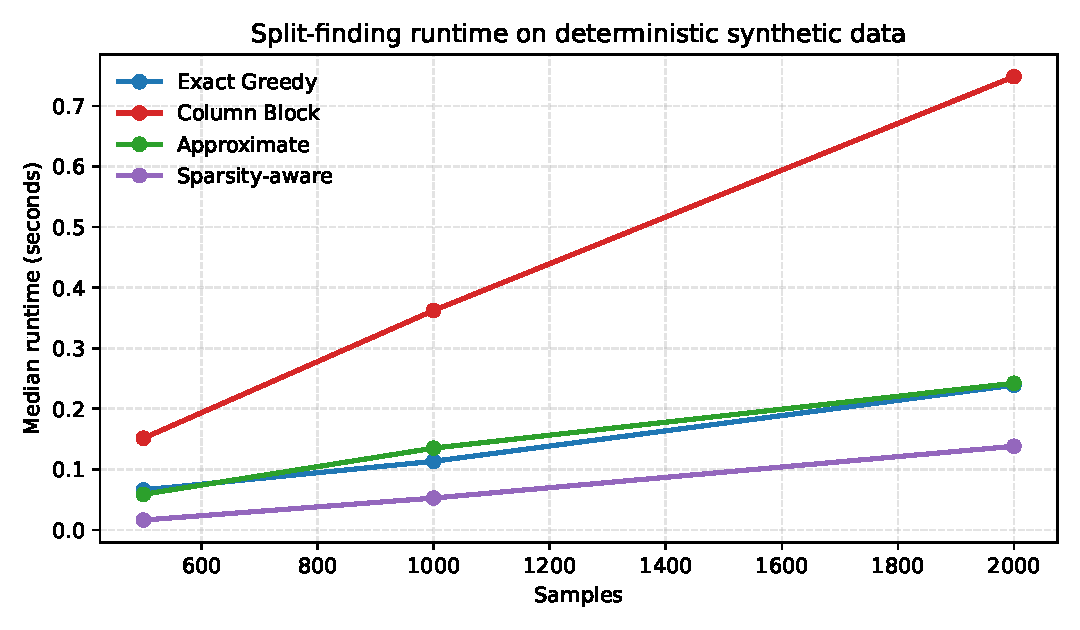
\includegraphics[width=0.82\textwidth]{images/runtime_comparison.pdf}
    \caption{So sánh runtime median giữa các thuật toán split finding}
    \label{fig:runtime_comparison}
\end{figure}

\subsection{Số candidate và gain}

Ngoài runtime, benchmark cũng ghi lại số candidate split được xét xấp xỉ và gain của split tốt nhất. Với $n=2000$ và $d=8$:

\begin{itemize}
    \item Exact Greedy và Column Block xét khoảng $15{,}992$ candidate trên dữ liệu dense.
    \item Approximate chỉ xét $160$ candidate do $\epsilon = 0.05$.
    \item Sparsity-aware xét khoảng $3{,}046$ candidate trên dữ liệu có $80\%$ missing.
\end{itemize}

Gain của Approximate thường nhỏ hơn Exact Greedy vì nhiều threshold bị bỏ qua. Đây là đánh đổi cốt lõi của approximate split finding: giảm chi phí bằng cách chấp nhận khả năng bỏ lỡ split tốt nhất.

\subsection{Nhận xét từ benchmark}

Kết quả cho thấy ba điểm chính.

Thứ nhất, Sparsity-aware Split Finding nhanh nhất trong benchmark này vì dữ liệu sparse chỉ có khoảng $20\%$ giá trị non-missing. Điều này phù hợp với phân tích độ phức tạp: khi số entry được scan giảm mạnh, thời gian chạy cũng giảm.

Thứ hai, Approximate Split Finding giảm rất mạnh số candidate. Tuy nhiên, bản Python hiện tại vẫn phải chia lại tập dữ liệu cho từng candidate, nên tốc độ chỉ nhỉnh hơn Exact Greedy trong một số cấu hình nhỏ. Trong cài đặt tối ưu hơn, các thống kê theo bucket có thể giúp tận dụng tốt hơn lợi thế $q \ll n$.

Thứ ba, Column Block trong benchmark này chậm hơn Exact Greedy. Nguyên nhân đến từ chi phí phụ của bản minh họa Python: lọc active row, cấp phát danh sách tạm và tạo thứ tự giảm dần khi xét default direction. Vì vậy, benchmark này không nên được dùng để kết luận rằng Column Block là chậm; nó chỉ cho thấy bản cài đặt hiện tại chưa tối ưu ở mức hệ thống.

\subsection{Liên hệ với phân tích độ phức tạp}

Thực nghiệm củng cố một thông điệp quan trọng: cùng một ý tưởng thuật toán có thể cho kết quả khác nhau tùy mức độ tối ưu của cài đặt.

Ở mức lý thuyết, Exact Greedy tốn chi phí vì xét gần như toàn bộ threshold, Approximate giảm số candidate, Sparsity-aware giảm số entry cần scan, và Column Block giảm việc sort lặp lại. Ở mức code Python minh họa, lợi ích này chỉ thể hiện rõ nhất với Sparsity-aware, trong khi Approximate và Column Block vẫn chịu overhead đáng kể.

Do đó, khi đọc benchmark, cần tách hai lớp kết luận:

\begin{itemize}
    \item \textbf{Kết luận thuật toán}: các kỹ thuật của XGBoost giảm chi phí bằng cách giảm sort, giảm candidate hoặc giảm entry scan.
    \item \textbf{Kết luận implementation}: bản Python trong repository minh họa đúng ý tưởng, nhưng chưa tối ưu như hệ thống XGBoost thật.
\end{itemize}

\section{Conclusion}

\subsection{Tổng kết}

Báo cáo đã trình bày quá trình phát triển từ cây quyết định (Decision Tree) đến các phương pháp học tổ hợp (Ensemble Learning), Gradient Boosting và cuối cùng là XGBoost.

Trước hết, báo cáo giới thiệu cây quyết định như một mô hình học máy có khả năng mô hình hóa các quan hệ phi tuyến và dễ diễn giải. Tuy nhiên, một cây đơn lẻ thường có độ chính xác hạn chế và dễ bị overfitting. Để khắc phục nhược điểm này, các phương pháp Ensemble Learning được đề xuất nhằm kết hợp nhiều mô hình yếu để tạo thành một mô hình mạnh hơn.

Tiếp theo, báo cáo trình bày Gradient Boosting, trong đó các cây được xây dựng tuần tự để giảm dần sai số dự đoán thông qua thông tin gradient của hàm mất mát. Trên nền tảng đó, XGBoost mở rộng Gradient Boosting bằng cách bổ sung regularization, khai triển Taylor bậc hai và nhiều tối ưu hóa ở mức thuật toán cũng như hệ thống.

Trọng tâm của báo cáo là phân tích các kỹ thuật tìm split trong XGBoost, bao gồm Exact Greedy Split, Column Block Structure, Approximate Split Finding, Weighted Quantile Sketch và Sparsity-aware Split Finding. Các kỹ thuật này tạo nên nền tảng giúp XGBoost đạt được hiệu năng cao trong thực tế.

\subsection{Nhận xét về độ phức tạp}

Từ góc nhìn của môn Nhập môn Phân tích độ phức tạp thuật toán, chi phí xây dựng cây chủ yếu đến từ quá trình tìm split. Nếu sử dụng phương pháp Exact Greedy Split, thuật toán phải xét một số lượng lớn candidate split, dẫn đến chi phí tính toán đáng kể khi dữ liệu có nhiều mẫu hoặc nhiều thuộc tính.

Các cải tiến của XGBoost đều hướng đến mục tiêu giảm chi phí này:

\begin{itemize}
    \item Column Block Structure loại bỏ việc sắp xếp lặp lại dữ liệu.
    \item Approximate Split Finding giảm số lượng candidate split cần xét.
    \item Weighted Quantile Sketch giúp lựa chọn candidate chất lượng hơn dựa trên thông tin Hessian.
    \item Sparsity-aware Split Finding tận dụng đặc tính sparse của dữ liệu và xử lý missing value hiệu quả.
\end{itemize}

Nhờ sự kết hợp của các kỹ thuật trên, XGBoost có khả năng mở rộng tốt trên các tập dữ liệu lớn trong khi vẫn duy trì chất lượng dự đoán cao.

\subsection{Hướng phát triển}

Trong tương lai, có thể mở rộng công việc theo một số hướng sau:

\begin{itemize}
    \item Triển khai đầy đủ các thuật toán và thực hiện thực nghiệm trên các bộ dữ liệu thực tế có quy mô lớn hơn.
    \item Nghiên cứu ảnh hưởng của các siêu tham số như \texttt{max\_depth}, \texttt{min\_child\_weight}, \texttt{gamma} và \texttt{learning\_rate} đến hiệu năng của XGBoost.
    \item So sánh XGBoost với các thư viện Gradient Boosting hiện đại khác như LightGBM và CatBoost dưới góc nhìn độ phức tạp và hiệu năng thực nghiệm.
    \item Tìm hiểu sâu hơn các tối ưu hóa ở mức hệ thống như cache-aware access, compression và distributed training trong XGBoost.
\end{itemize}

Qua quá trình tìm hiểu, có thể thấy rằng thành công của XGBoost không chỉ đến từ mô hình Gradient Boosting mà còn đến từ việc thiết kế các thuật toán và cấu trúc dữ liệu hiệu quả, giúp giảm đáng kể chi phí tính toán trong quá trình huấn luyện.

\newpage
\bibliographystyle{ieeetr}
\bibliography{references}

\end{document}
